\documentclass[a4paper]{article}

% Version: $Revision: 1.11 $

\usepackage{epsfig}

\title{
\epsfig{file=images/coat_of_arms.eps,width=10cm}\vspace{3cm}\\WEKA Experimenter Tutorial\\for Version 3-5-8}
\author{David Scuse\\Peter Reutemann}

\setcounter{secnumdepth}{3}
\setcounter{tocdepth}{3}

% hyphenation stuff
\hyphenation{Generic-Object-Editor}
\hyphenation{Result-Producer}
\hyphenation{Cross-Validation-Result-Producer}
\hyphenation{Random-Split-Result-Producer}
\hyphenation{Database-Result-Listener}
\hyphenation{DatabaseUtils}

\begin{document}

\begin{titlepage}

\maketitle
\thispagestyle{empty}

\center
\vspace{8cm}

\copyright 2002-2008 David Scuse and University of Waikato

\end{titlepage}

\tableofcontents

%%%%%%%%%%%%%%%%
% Introduction %
%%%%%%%%%%%%%%%%

\newpage
\section{Introduction}

The Weka Experiment Environment enables the user to create, run, modify, and analyse experiments in a more convenient manner than is possible when processing the schemes individually. For example, the user can create an experiment that runs several schemes against a series of datasets and then analyse the results to determine if one of the schemes is (statistically) better than the other schemes.

The Experiment Environment can be run from the command line using the Simple CLI. For example, the following commands could be typed into the CLI to run the \texttt{OneR} scheme on the Iris dataset using a basic train and test process. (Note that the commands would be typed on one line into the CLI.)

\begin{verbatim}
java weka.experiment.Experiment -r -T data/iris.arff
  -D weka.experiment.InstancesResultListener
  -P weka.experiment.RandomSplitResultProducer --
  -W weka.experiment.ClassifierSplitEvaluator --
  -W weka.classifiers.rules.OneR
\end{verbatim}

While commands can be typed directly into the CLI, this technique is not particularly convenient and the experiments are not easy to modify.

The Experimenter comes in two flavours, either with a simple interface that provides most of the functionality one needs for experiments, or with an interface with full access to the Experimenter's capabilities. You can choose between those two with the \textit{Experiment Configuration Mode} radio buttons:

\begin{itemize}
	\item Simple
	\item Advanced 
\end{itemize}

Both setups allow you to setup \textit{standard} experiments, that are run locally on a single machine, or remote experiments, which are distributed between several hosts. The distribution of experiments cuts down the time the experiments will take until completion, but on the other hand the setup takes more time.

The next section covers the \textit{standard} experiments (both, simple and advanced), followed by the \textit{remote} experiments and finally the \textit{analysing} of the results.

This manual is also available online on the \textit{WekaDoc Wiki} \cite{wekadoc}.

%%%%%%%%%%%%%%%%%%%%%%%%
% Standard Experiments %
%%%%%%%%%%%%%%%%%%%%%%%%

\newpage
\section{Standard Experiments}

%%%%%%%%%%
% Simple %
%%%%%%%%%%

\subsection{Simple}

\subsubsection{New experiment}

After clicking \textit{New} default parameters for an Experiment are defined.

\begin{center}
	\epsfig{file=images/simple_new.eps,width=10cm}
\end{center}


\subsubsection{Results destination}

By default, an ARFF file is the destination for the results output. But you can choose between

\begin{itemize}
	\item ARFF file
   \item CSV file
   \item JDBC database 
\end{itemize}

ARFF file and JDBC database are discussed in detail in the following sections. CSV is similar to ARFF, but it can be used to be loaded in an external spreadsheet application.


\subsubsection*{ARFF file}

If the file name is left empty a temporary file will be created in the TEMP directory of the system. If one wants to specify an explicit results file, click on \textit{Browse} and choose a filename, e.g., \textit{Experiment1.arff}.

\begin{center}
	\epsfig{file=images/simple_saveoutput_ARFF1.eps,width=7cm}
\end{center}


Click on \textit{Save} and the name will appear in the edit field next to \textit{ARFF file}.

\begin{center}
	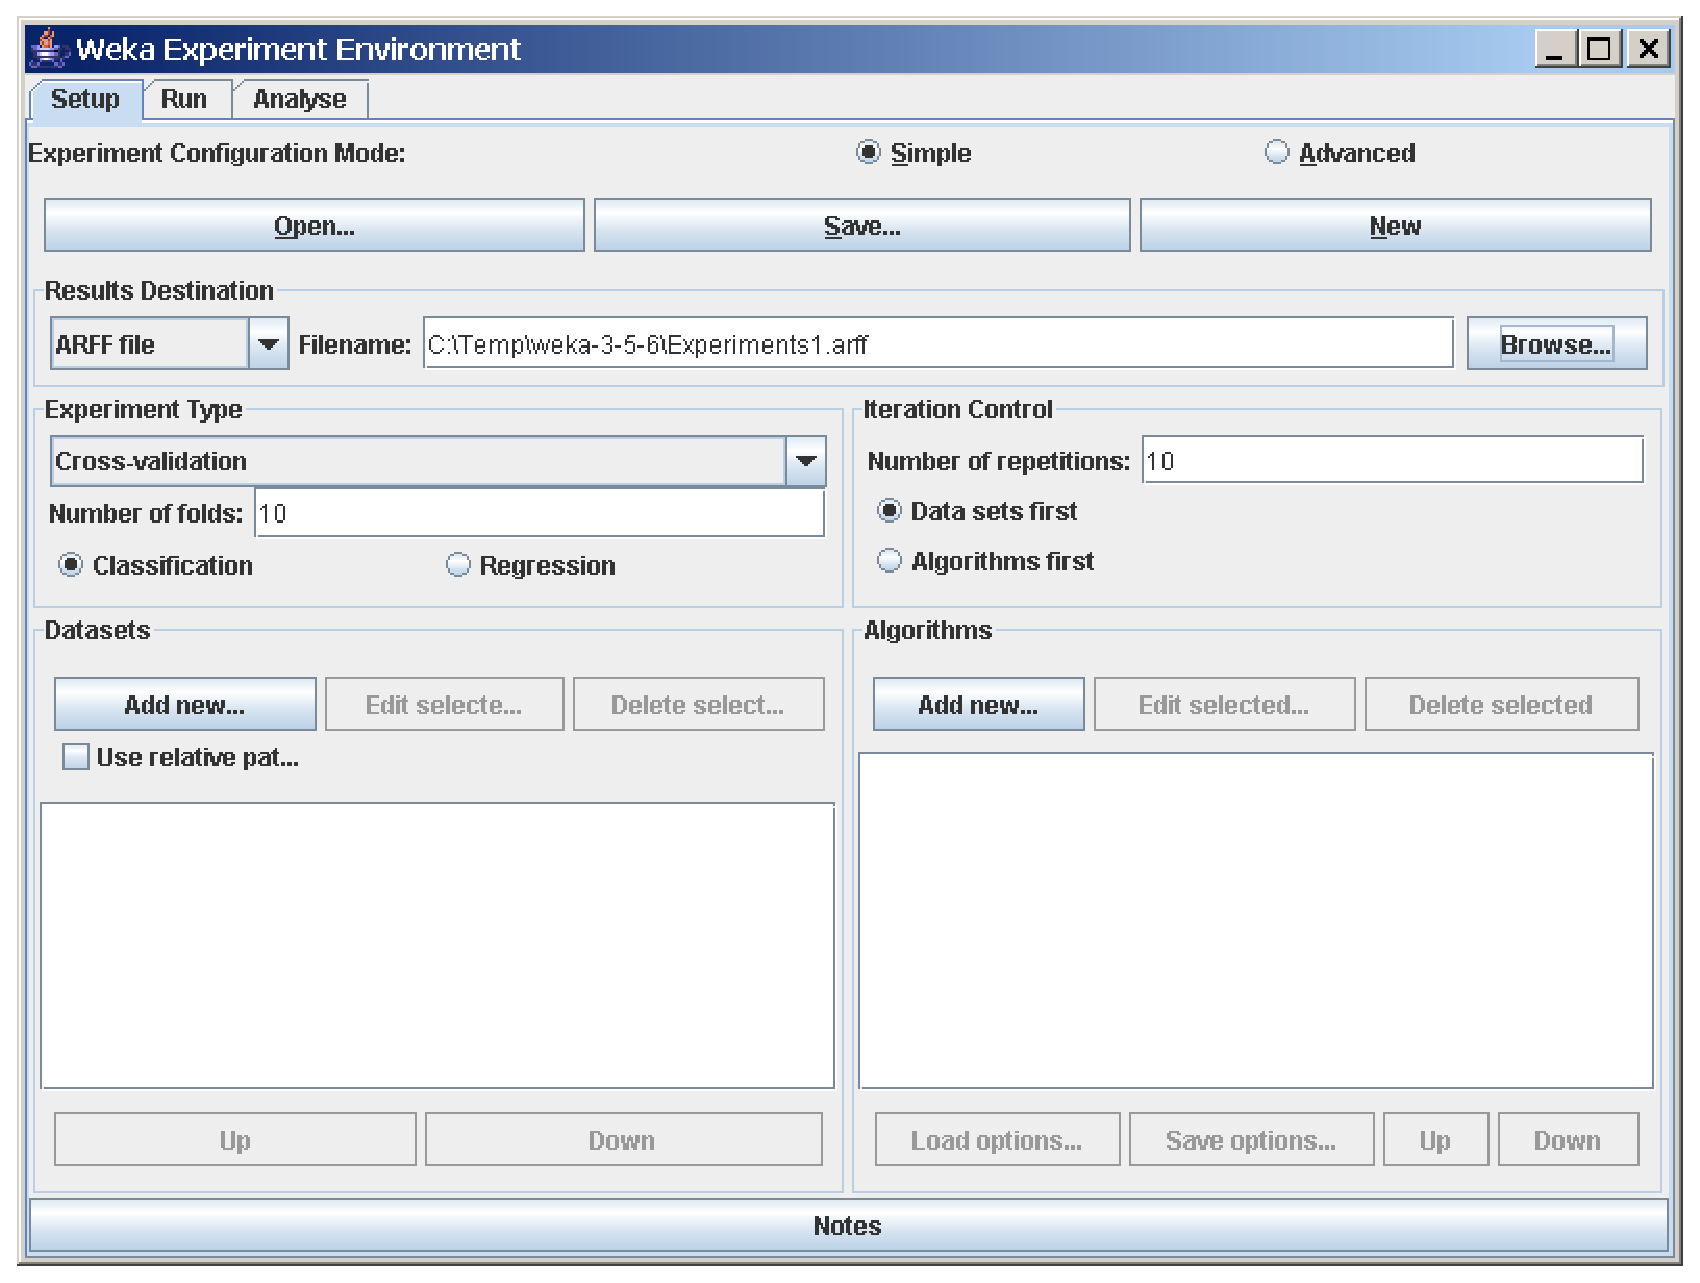
\epsfig{file=images/simple_saveoutput_ARFF2.eps,width=10cm}
\end{center}


The advantage of ARFF or CSV files is that they can be created without any additional classes besides the ones from Weka. The drawback is the lack of the ability to resume an experiment that was interrupted, e.g., due to an error or the addition of dataset or algorithms. Especially with time-consuming experiments, this behavior can be annoying.


\subsubsection*{JDBC database}

With JDBC it is easy to store the results in a database. The necessary jar archives have to be in the CLASSPATH to make the JDBC functionality of a particular database available.

After changing \textit{ARFF file} to \textit{JDBC database} click on \textit{User...} to specify JDBC URL and user credentials for accessing the database.

\begin{center}
	\epsfig{file=images/simple_saveoutput_JDBC1.eps,width=8cm}
\end{center}


After supplying the necessary data and clicking on \textit{OK}, the URL in the main window will be updated.

\textit{Note:} at this point, the database connection is not tested; this is done when the experiment is started.

\begin{center}
	\epsfig{file=images/simple_saveoutput_JDBC2.eps,width=10cm}
\end{center}


The advantage of a JDBC database is the possibility to resume an interrupted or extended experiment. Instead of re-running all the other algorithm/dataset combinations again, only the missing ones are computed.


\subsubsection{Experiment type}

The user can choose between the following three different types

\begin{itemize}
	\item \textbf{Cross-validation (default)} \\
      performs stratified cross-validation with the given number of folds 

   \item \textbf{Train/Test Percentage Split (data randomized)} \\
      splits a dataset according to the given percentage into a train and a test file (one cannot specify explicit training and test files in the Experimenter), after the order of the data has been randomized and stratified
	
	\begin{center}
		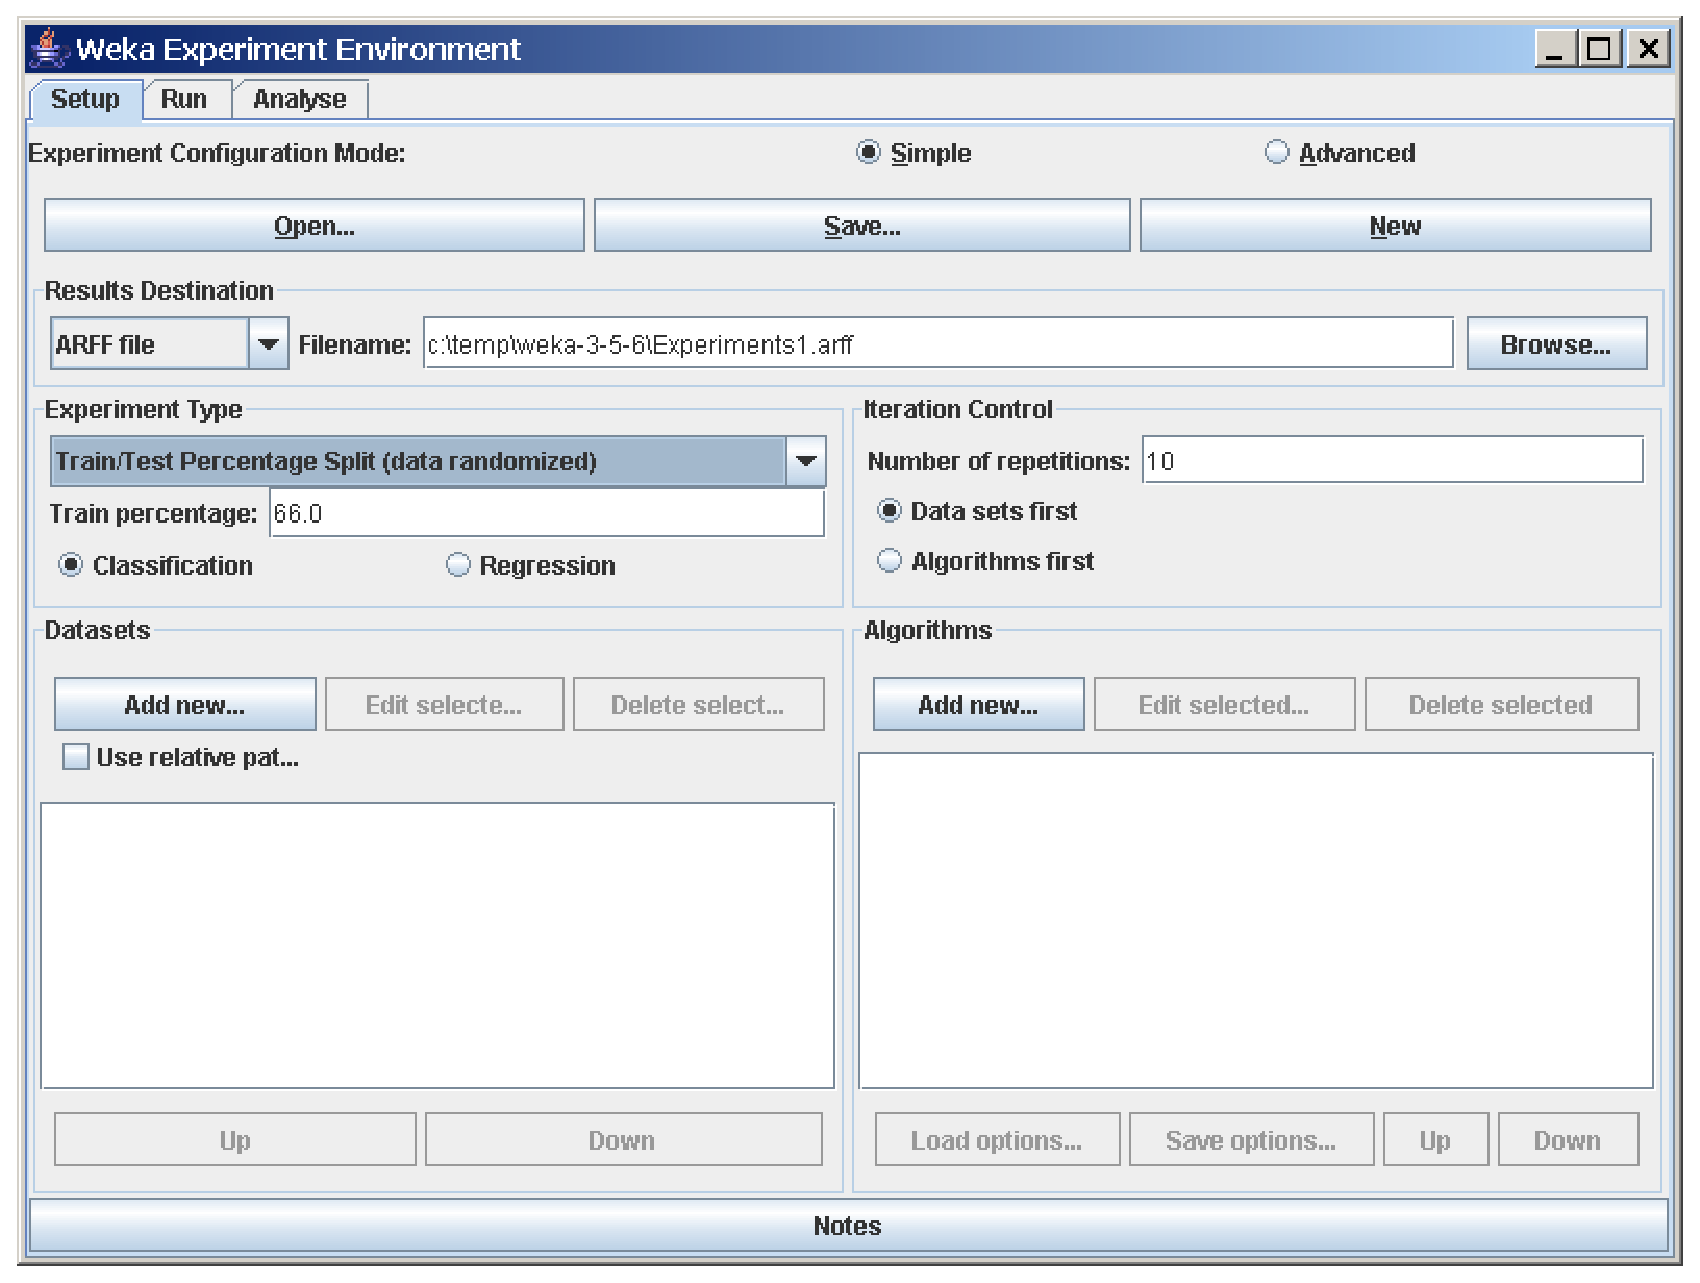
\epsfig{file=images/simple_experimenttype1.eps,width=10cm}
	\end{center}

    \item \textbf{Train/Test Percentage Split (order preserved)} \\
      because it is impossible to specify an explicit train/test files pair, one can \textit{abuse} this type to \textit{un-merge} previously merged train and test file into the two original files (one only needs to find out the correct percentage) 
	
	\begin{center}
		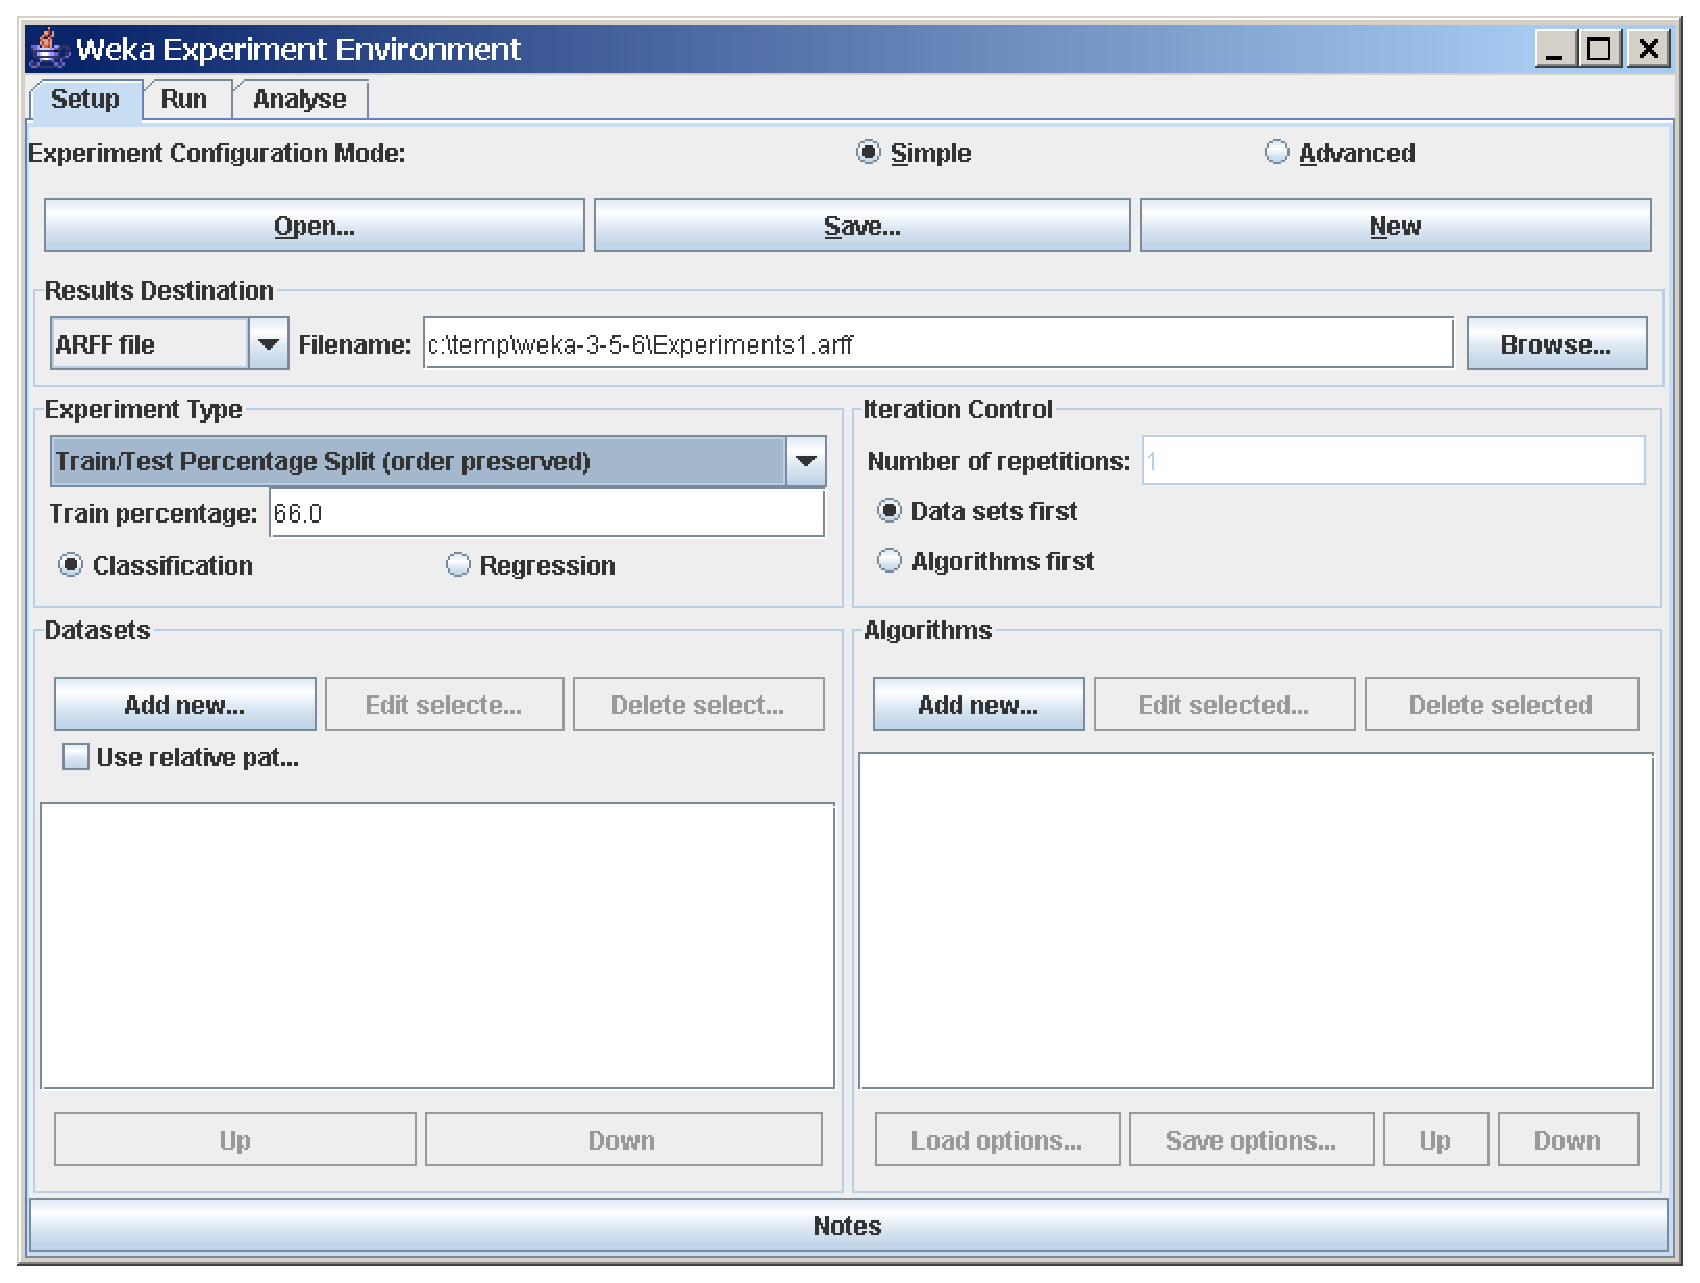
\epsfig{file=images/simple_experimenttype2.eps,width=10cm}
	\end{center}
	
\end{itemize}

Additionally, one can choose between \textit{Classification} and \textit{Regression}, depending on the datasets and classifiers one uses. For decision trees like \texttt{J48} (Weka's implementation of Quinlan's C4.5 \cite{quinlan}) and the iris dataset, \textit{Classification} is necessary, for a numeric classifier like \texttt{M5P}, on the other hand, \textit{Regression}. \textit{Classification} is selected by default.

\textit{Note:} if the percentage splits are used, one has to make sure that the corrected paired \textit{T-Tester} still produces sensible results with the given ratio \cite{bengio}.


\subsubsection{Datasets}

One can add dataset files either with an absolute path or with a relative one. The latter makes it often easier to run experiments on different machines, hence one should check \textit{Use relative paths}, before clicking on \textit{Add new...}.

\begin{center}
	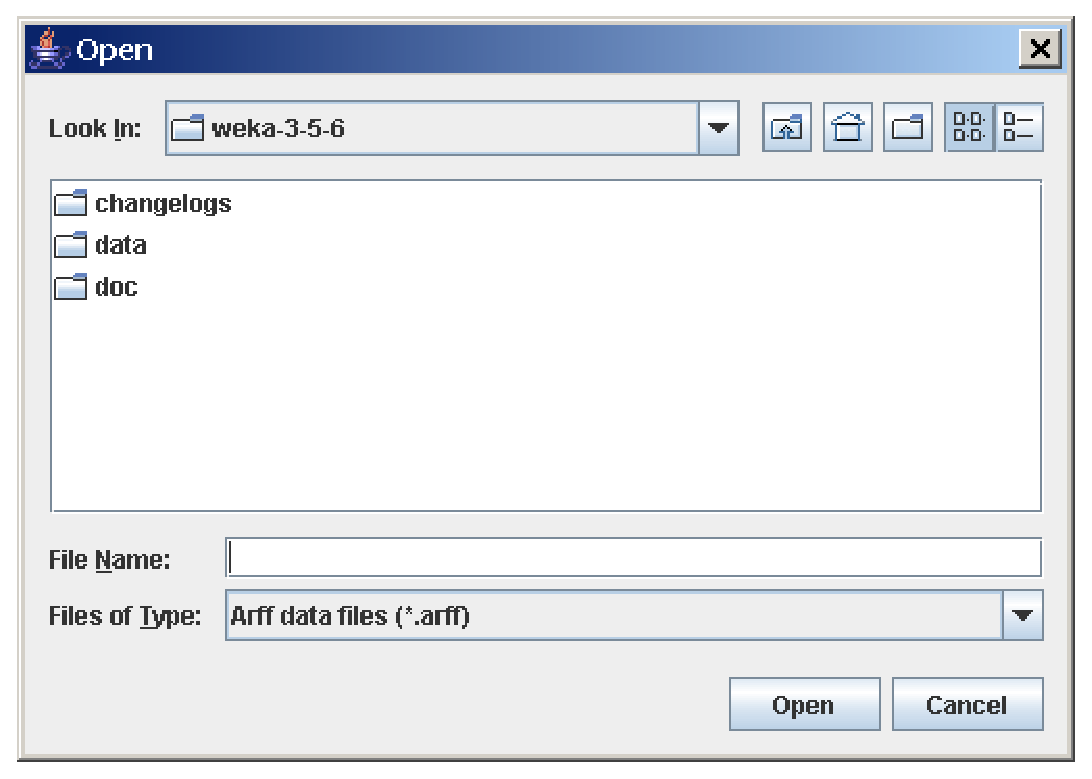
\epsfig{file=images/simple_adddataset1.eps,width=7cm}
\end{center}


In this example, open the \textit{data} directory and choose the \textit{iris.arff} dataset.

\begin{center}
	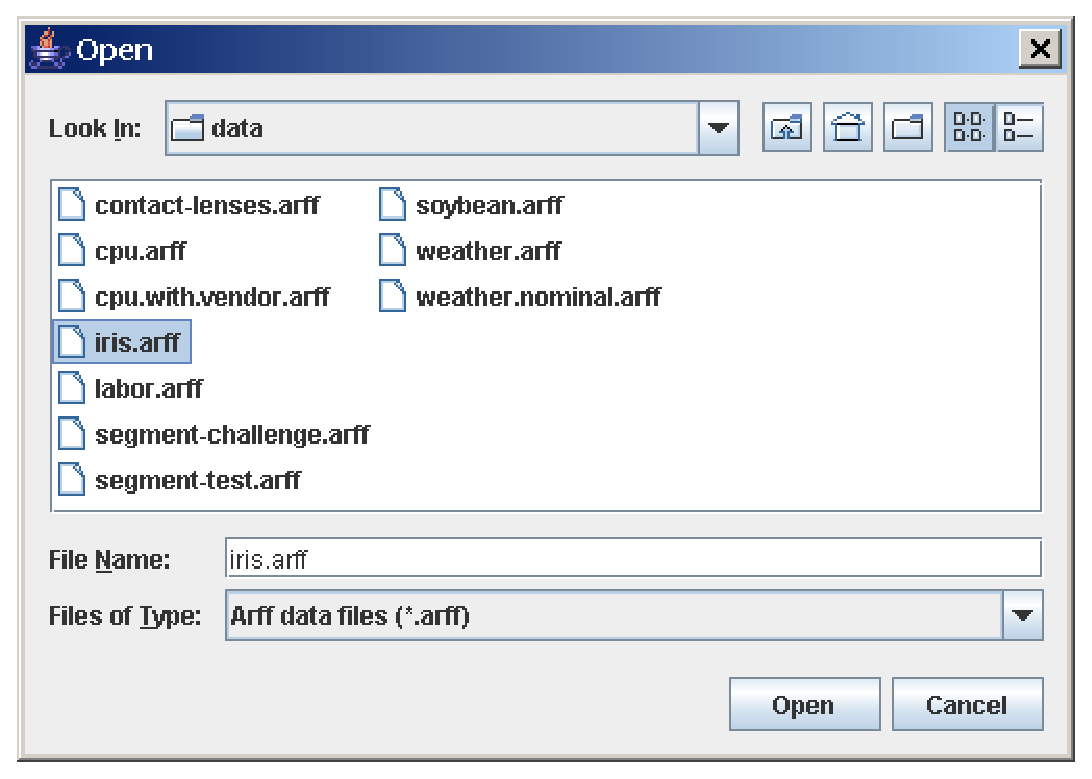
\epsfig{file=images/simple_adddataset2.eps,width=7cm}
\end{center}


After clicking \textit{Open} the file will be displayed in the datasets list. If one selects a directory and hits \textit{Open}, then all ARFF files will be added recursively. Files can be deleted from the list by selecting them and then clicking on \textit{Delete selected}.

ARFF files are not the only format one can load, but \textit{all} files that can be converted with Weka's \textit{``core converters''}. The following formats are currently supported:

\begin{itemize}
	\item ARFF (+ compressed)
	\item C4.5
	\item CSV
	\item libsvm
	\item binary serialized instances
	\item XRFF (+ compressed)
\end{itemize}

By default, the class attribute is assumed to be the last attribute. But if a data format contains information about the class attribute, like XRFF or C4.5, this attribute will be used instead.

\begin{center}
	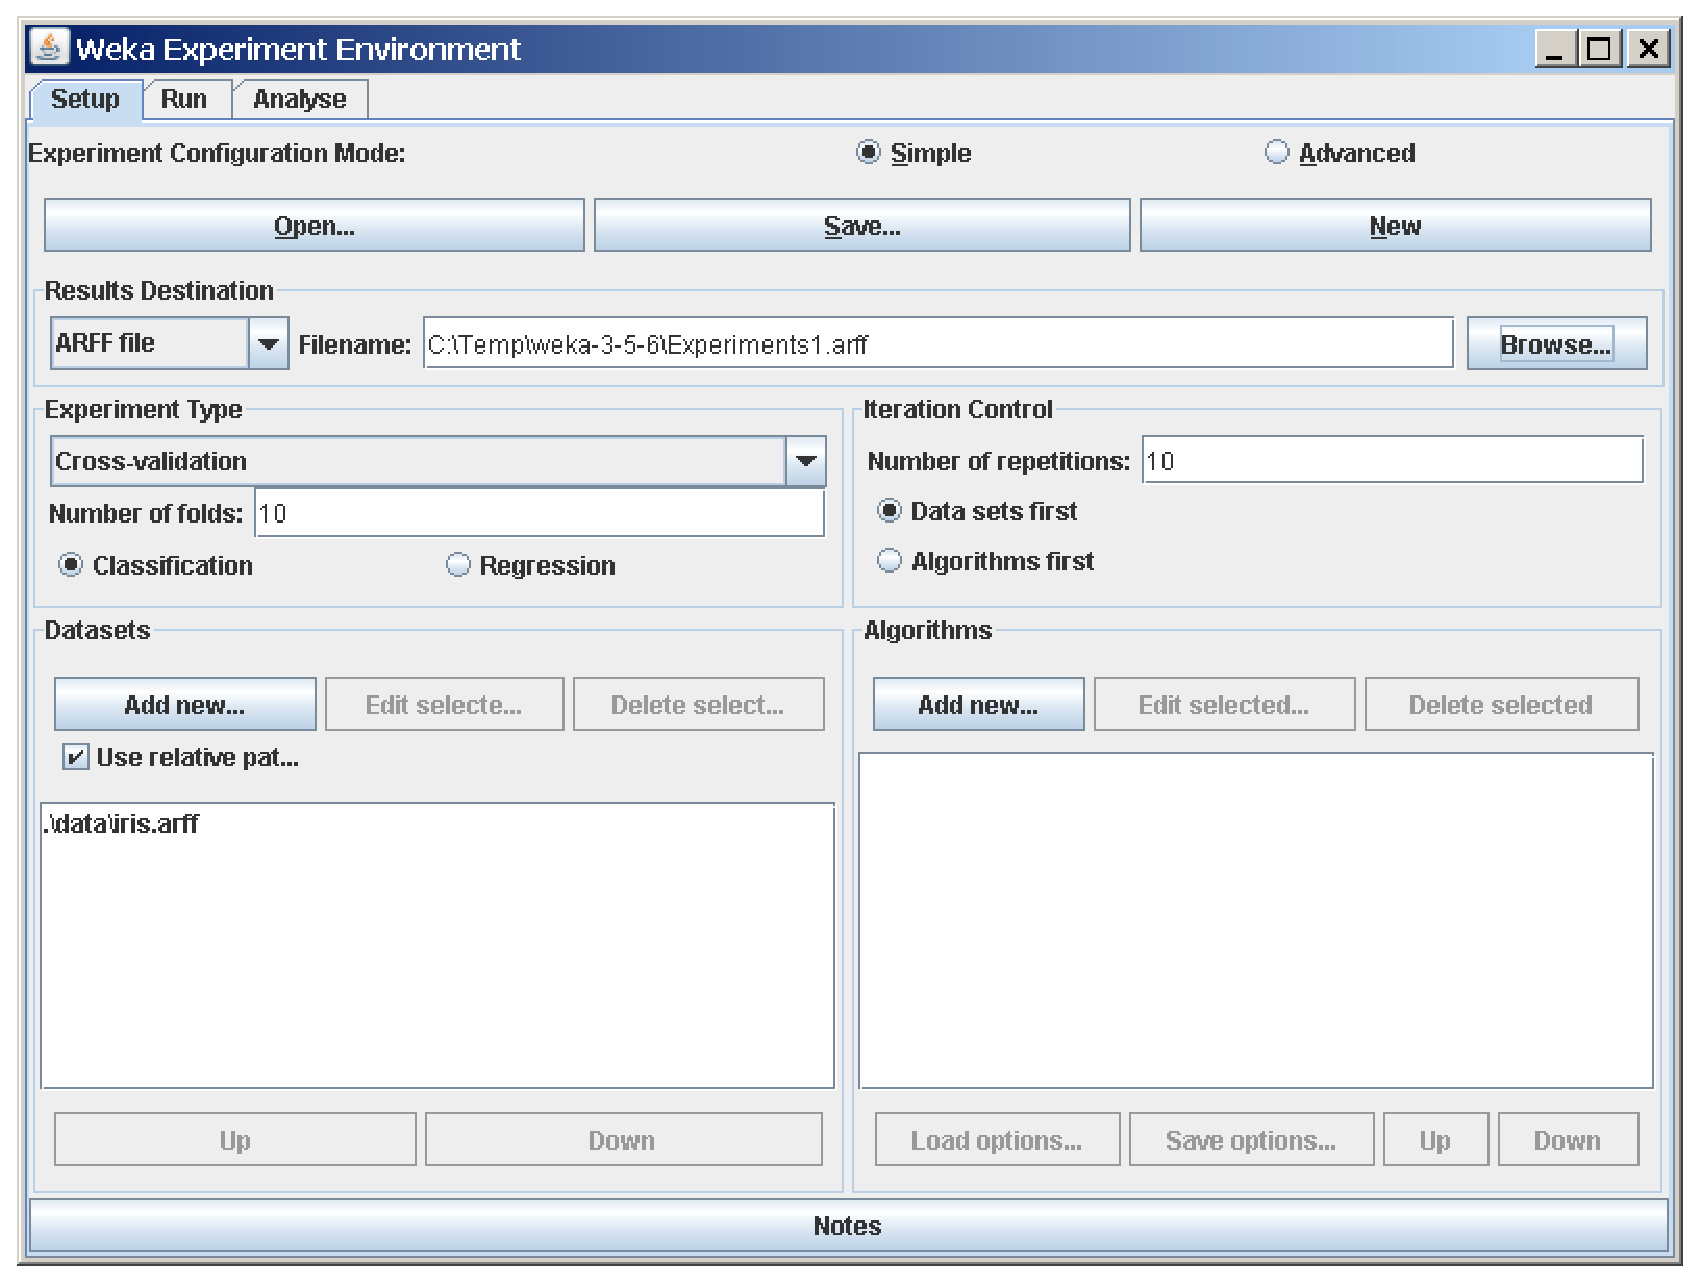
\epsfig{file=images/simple_adddataset3.eps,width=10cm}
\end{center}


\subsubsection{Iteration control}

\begin{itemize}
   \item \textbf{Number of repetitions} \\
      In order to get statistically meaningful results, the default number of iterations is 10. In case of 10-fold cross-validation this means 100 calls of one classifier with training data and tested against test data. 

   \item \textbf{Data sets first/Algorithms first} \\
      As soon as one has more than one dataset and algorithm, it can be useful to switch from datasets being iterated over first to algorithms. This is the case if one stores the results in a database and wants to complete the results for all the datasets for one algorithm as early as possible. 
\end{itemize}


\subsubsection{Algorithms}

New algorithms can be added via the \textit{Add new...} button. Opening this dialog for the first time, \texttt{ZeroR} is presented, otherwise the one that was selected last.

\begin{center}
	\epsfig{file=images/simple_addalgorithm1.eps,width=6cm}
\end{center}


With the \textit{Choose} button one can open the \textit{GenericObjectEditor} and choose another classifier.

\begin{center}
	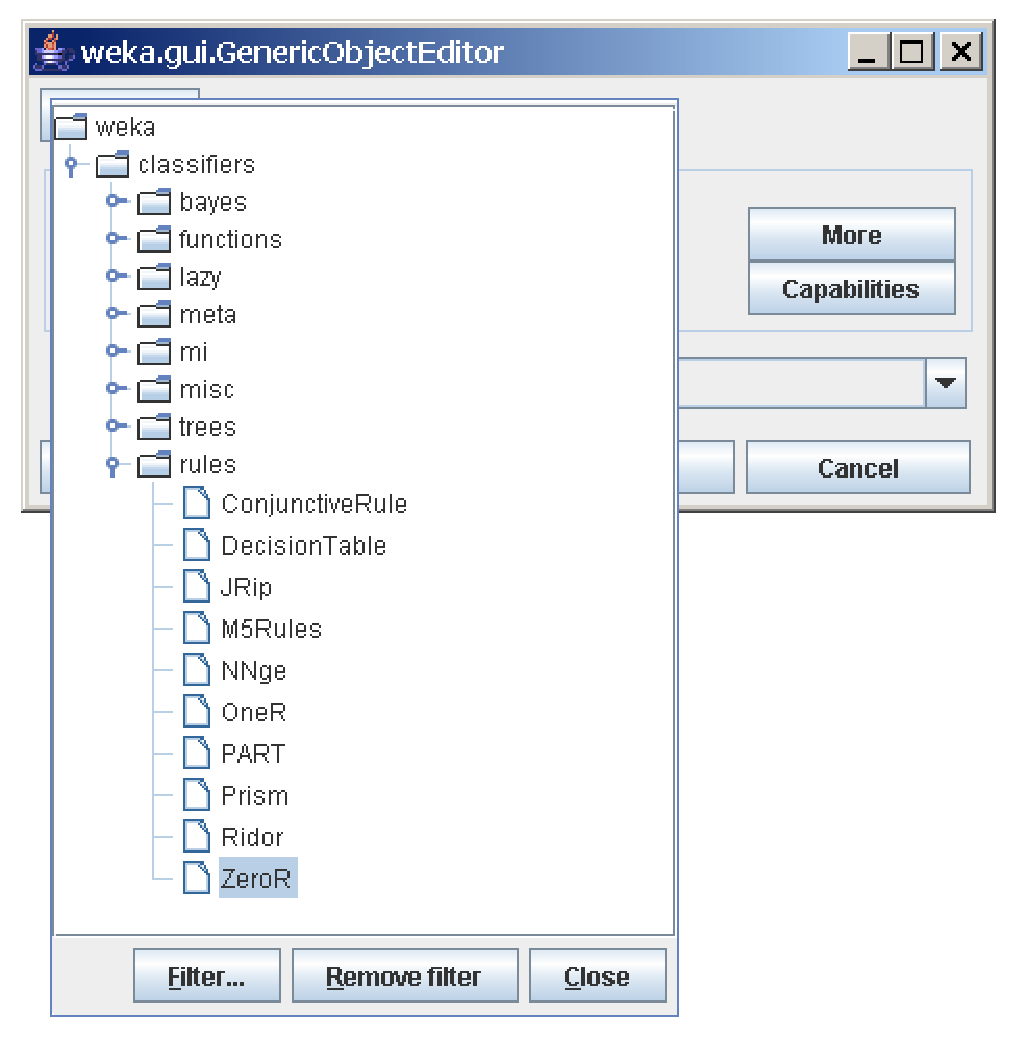
\epsfig{file=images/simple_addalgorithm2.eps,width=6cm}
\end{center}

The \textit{Filter...} button enables one to highlight classifiers that can handle certain attribute and class types. With the \textit{Remove filter} button all the selected capabilities will get cleared and the highlighting removed again.

Additional algorithms can be added again with the \textit{Add new...} button, e.g., the \texttt{J48} decision tree.

\begin{center}
	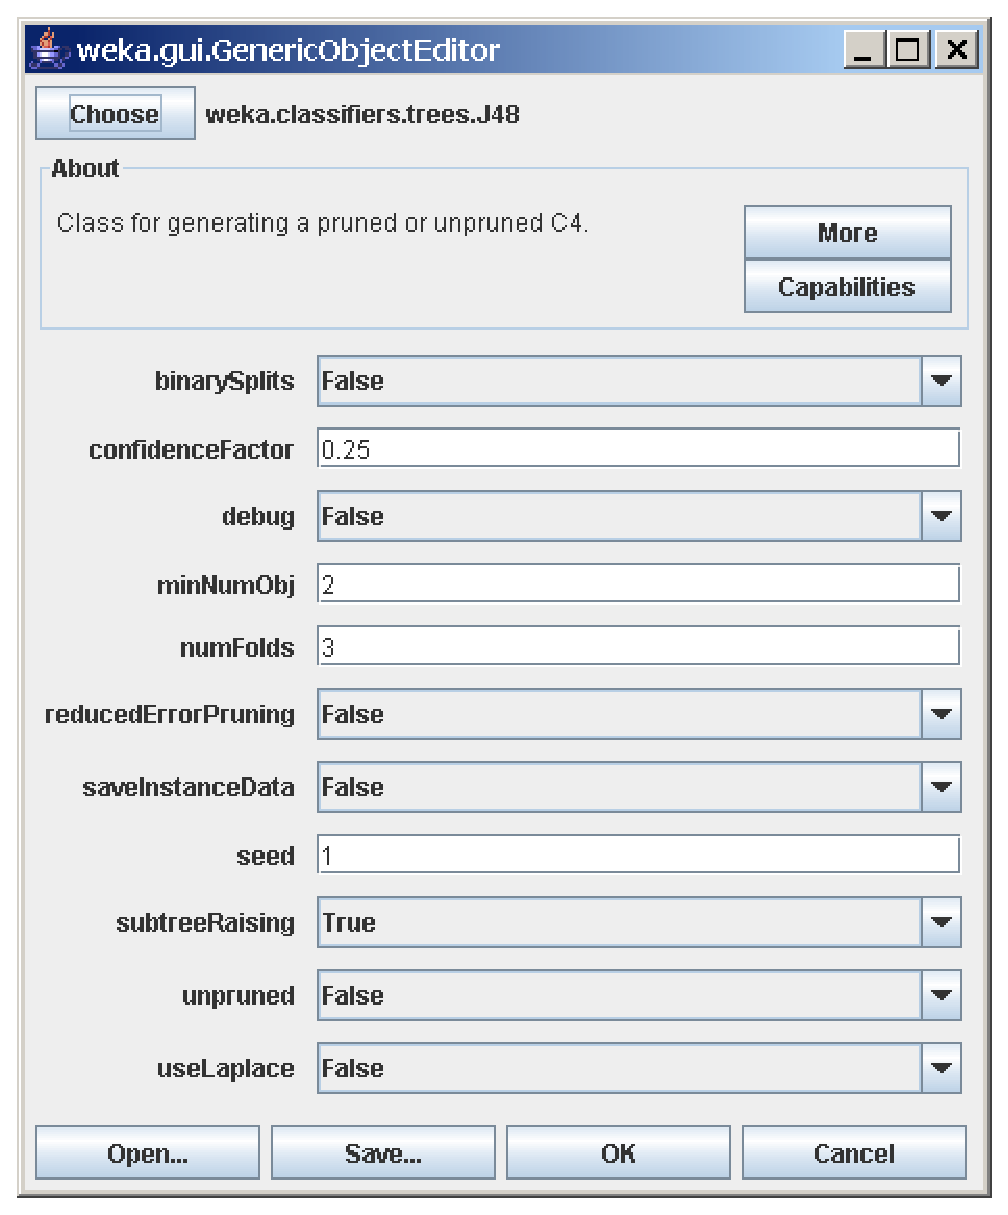
\epsfig{file=images/simple_addalgorithm3.eps,width=6cm}
\end{center}


After setting the classifier parameters, one clicks on \textit{OK} to add it to the list of algorithms.

\begin{center}
	\epsfig{file=images/simple_addalgorithm4.eps,width=10cm}
\end{center}


With the \textit{Load options...} and \textit{Save options...} buttons one can load and save the setup of a selected classifier from and to XML. This is especially useful for highly configured classifiers (e.g., nested meta-classifiers), where the manual setup takes quite some time, and which are used often.

One can also paste classifier settings here by right-clicking (or \textit{Alt-Shift-left-clicking}) and selecting the appropriate menu point from the popup menu, to either add a new classifier or replace the selected one with a new setup. This is rather useful for transferring a classifier setup from the Weka Explorer over to the Experimenter without having to setup the classifier from scratch.

\subsubsection{Saving the setup}

For future re-use, one can save the current setup of the experiment to a file by clicking on \textit{Save...} at the top of the window.

\begin{center}
	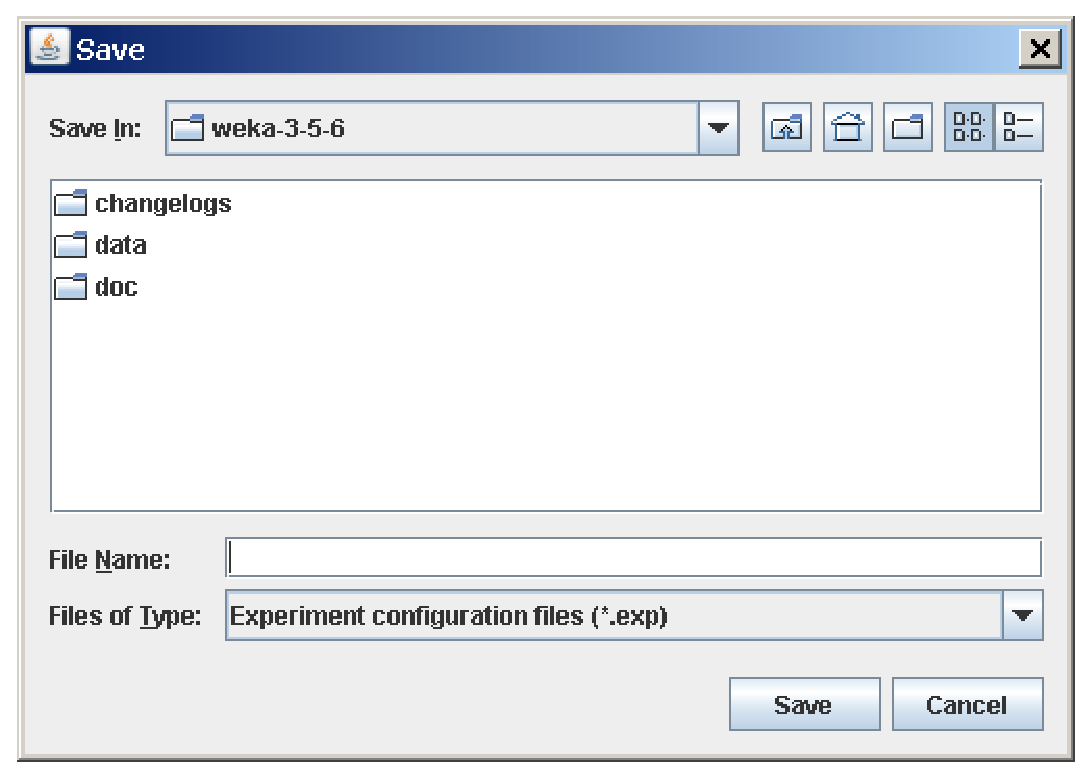
\epsfig{file=images/simple_save.eps,width=7cm}
\end{center}


By default, the format of the experiment files is the binary format that Java serialization offers. The drawback of this format is the possible incompatibility between different versions of Weka. A more robust alternative to the binary format is the XML format.

Previously saved experiments can be loaded again via the \textit{Open...} button.


\subsubsection{Running an Experiment}

To run the current experiment, click the \textit{Run} tab at the top of the Experiment Environment window. The current experiment performs 10 runs of 10-fold stratified cross-validation on the Iris dataset using the \texttt{ZeroR} and \texttt{J48} scheme.

\begin{center}
	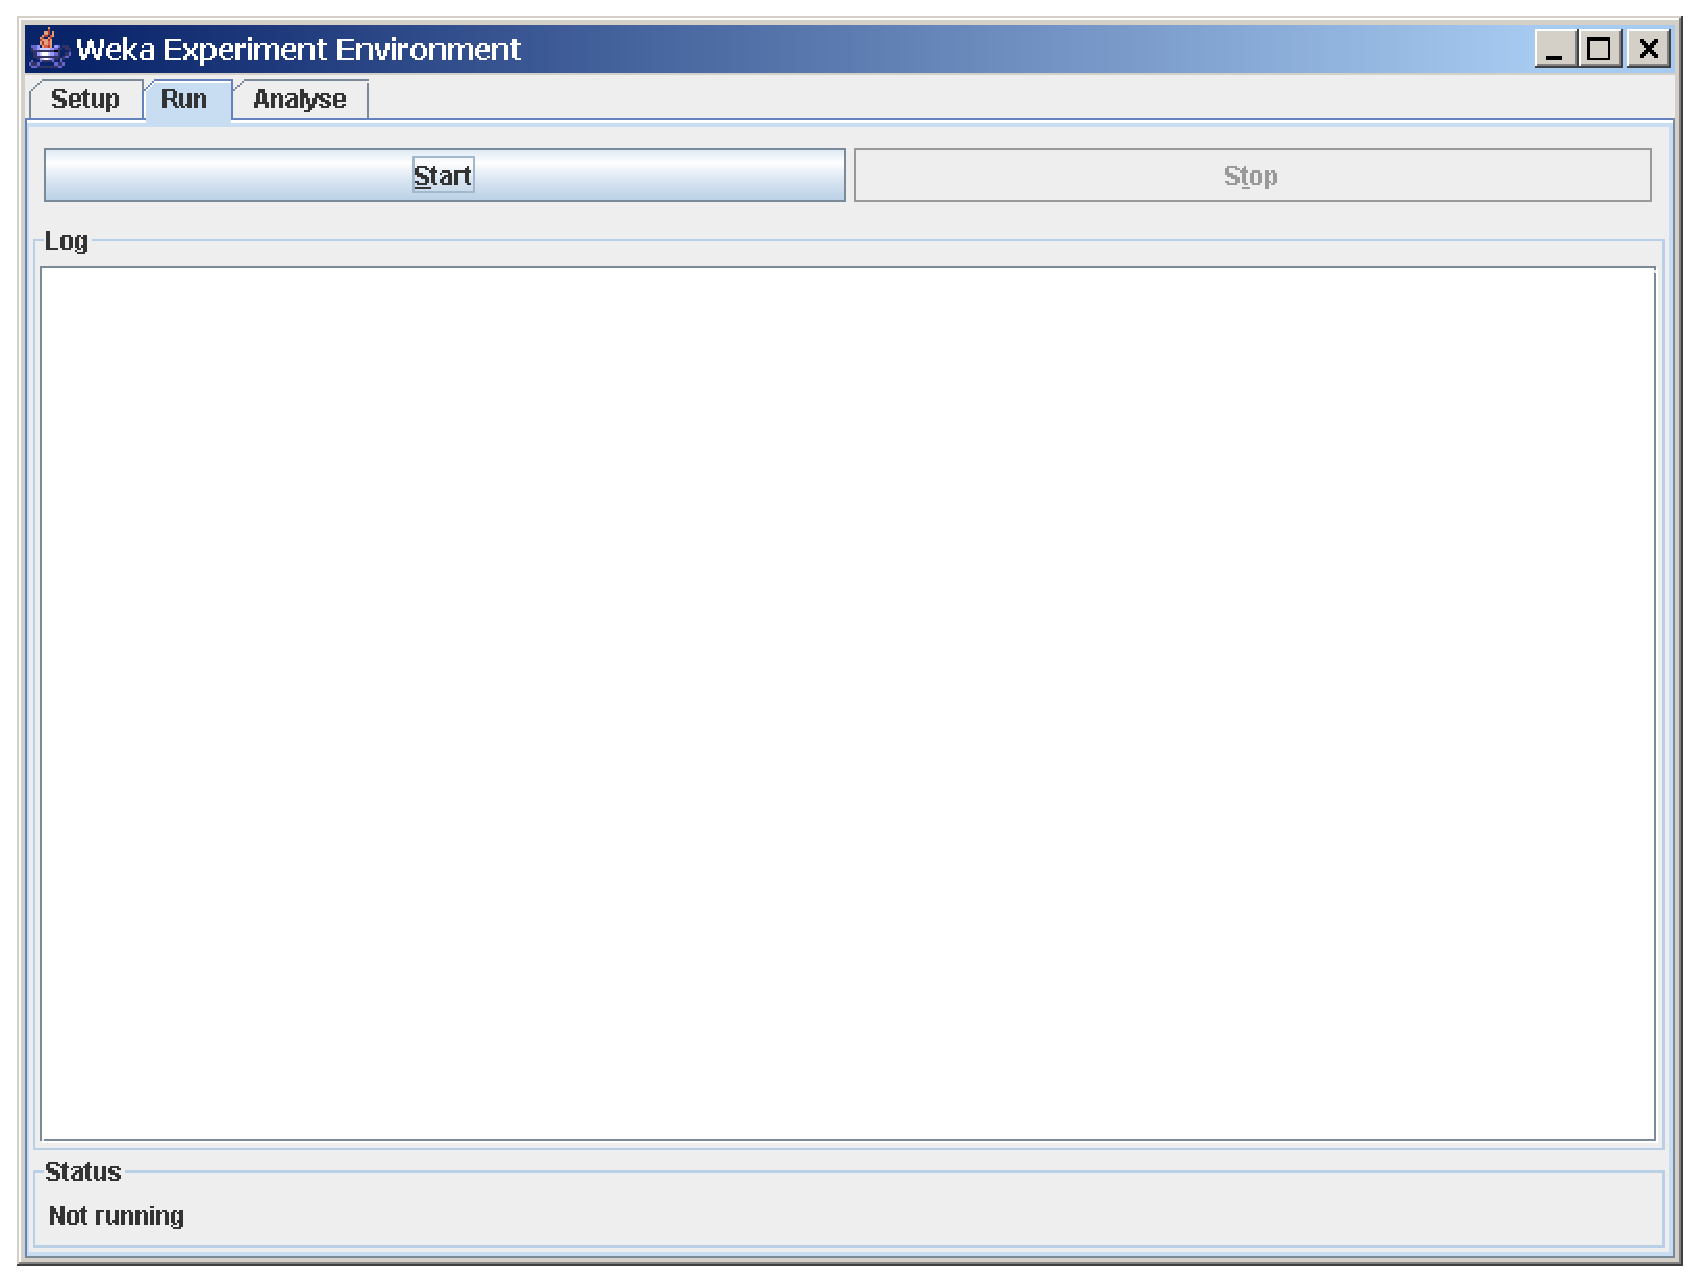
\epsfig{file=images/runexperiment1.eps,width=10cm}
\end{center}


Click \textit{Start} to run the experiment.

\begin{center}
	\epsfig{file=images/runexperiment2.eps,width=10cm}
\end{center}


If the experiment was defined correctly, the 3 messages shown above will be displayed in the \textit{Log} panel. The results of the experiment are saved to the dataset \textit{Experiment1.arff}. 

%%%%%%%%%%%%
% Advanced %
%%%%%%%%%%%%

\newpage
\subsection{Advanced}

\subsubsection{Defining an Experiment}

When the Experimenter is started in \textit{Advanced} mode, the \textit{Setup} tab is displayed. Click \textit{New} to initialize an experiment. This causes default parameters to be defined for the experiment.
\begin{center}
	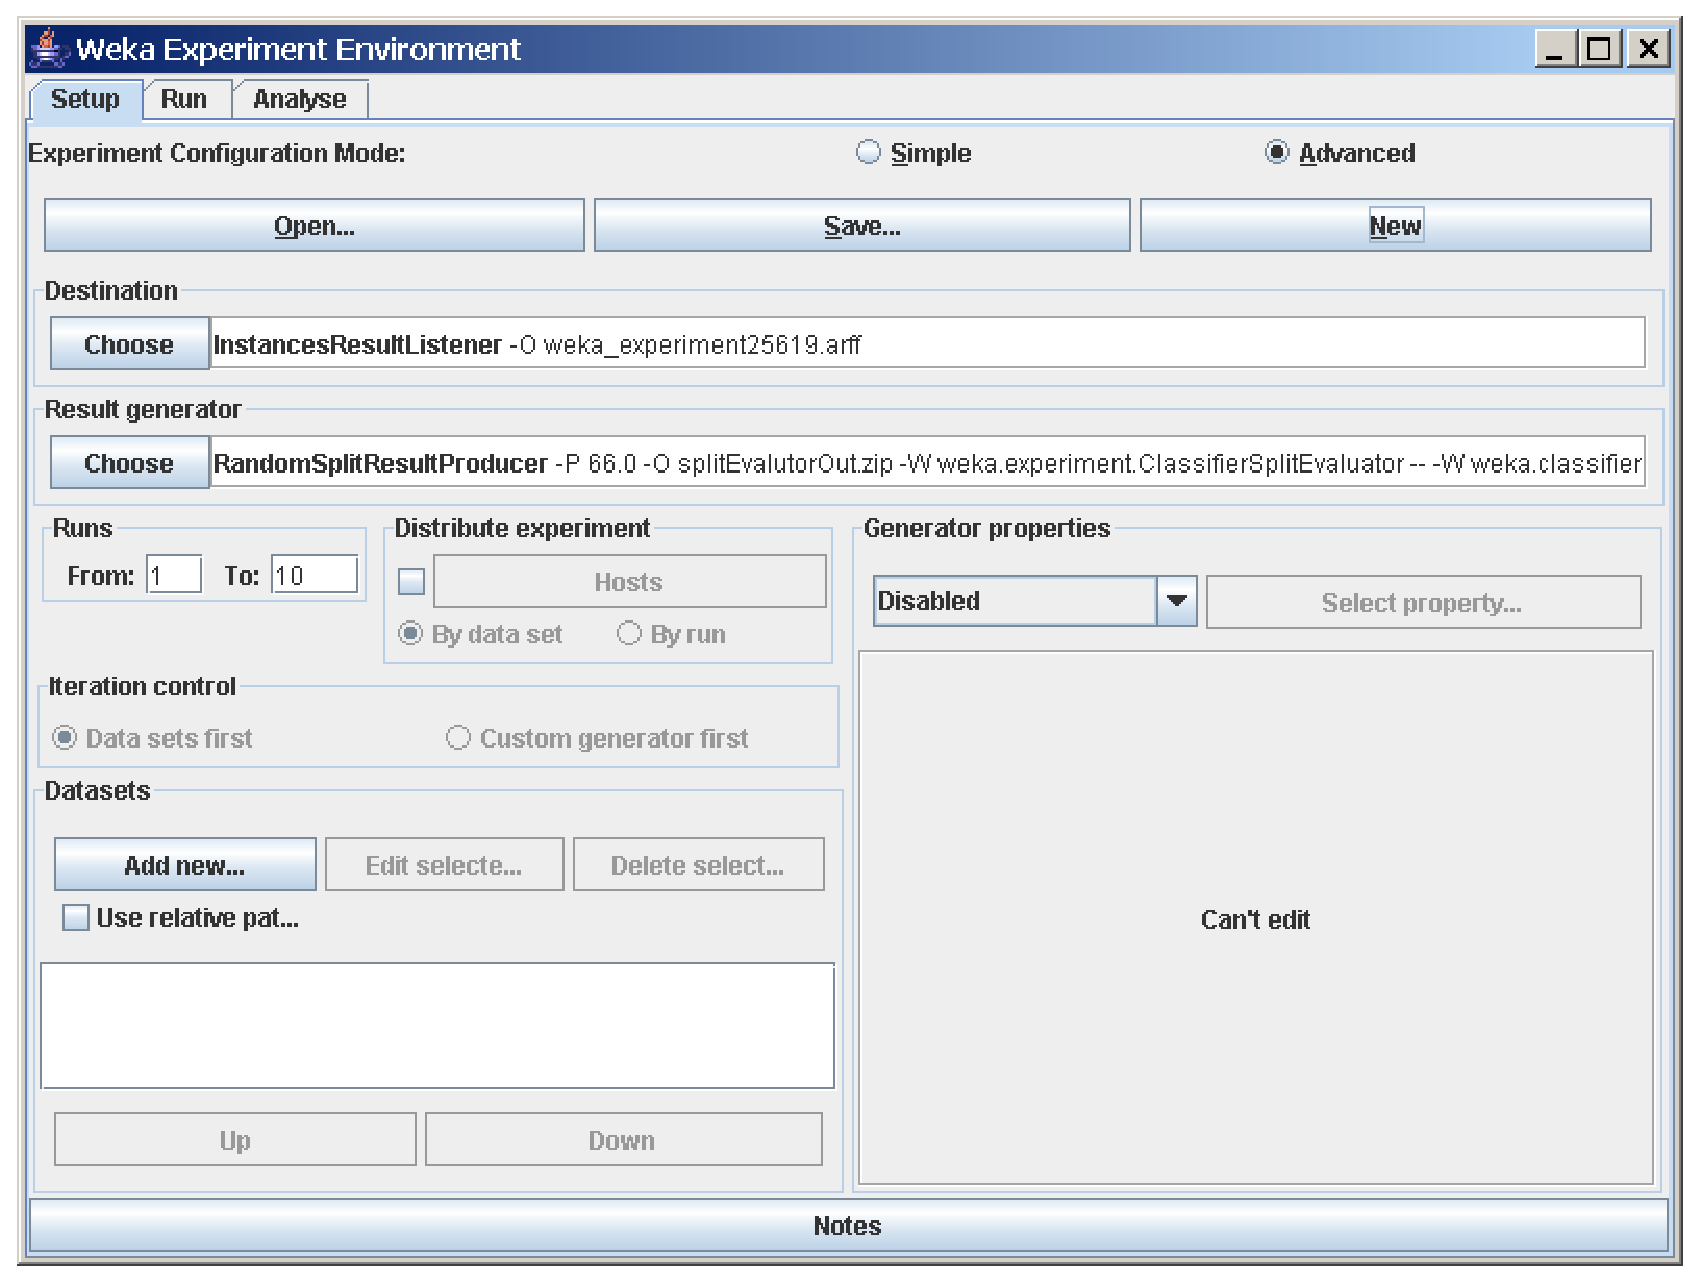
\epsfig{file=images/advanced_new.eps,width=10cm}
\end{center}

To define the dataset to be processed by a scheme, first select \textit{Use relative paths} in the \textit{Datasets} panel of the \textit{Setup} tab and then click on \textit{Add new...} to open a dialog window.
\begin{center}
	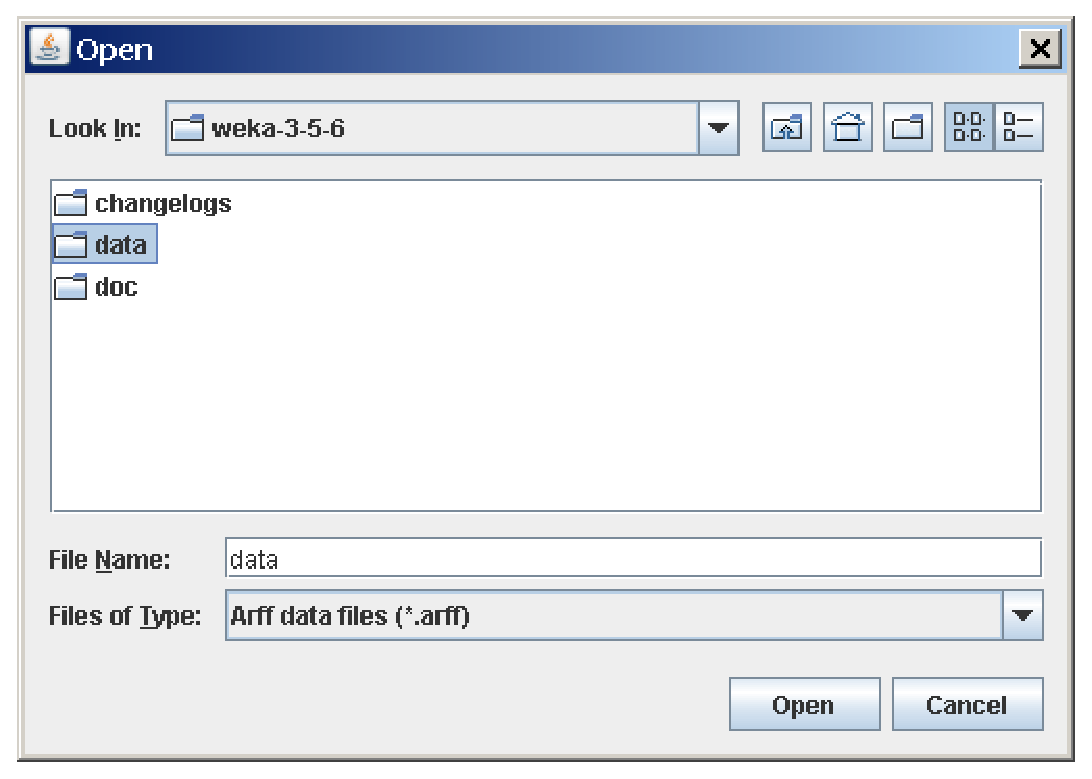
\epsfig{file=images/advanced_adddataset1.eps,width=7cm}
\end{center}

Double click on the \textit{data} folder to view the available datasets or navigate to an alternate location. Select \textit{iris.arff} and click \textit{Open} to select the Iris dataset.
\begin{center}
	\epsfig{file=images/advanced_adddataset2.eps,width=7cm}
\end{center}
	
\begin{center}
	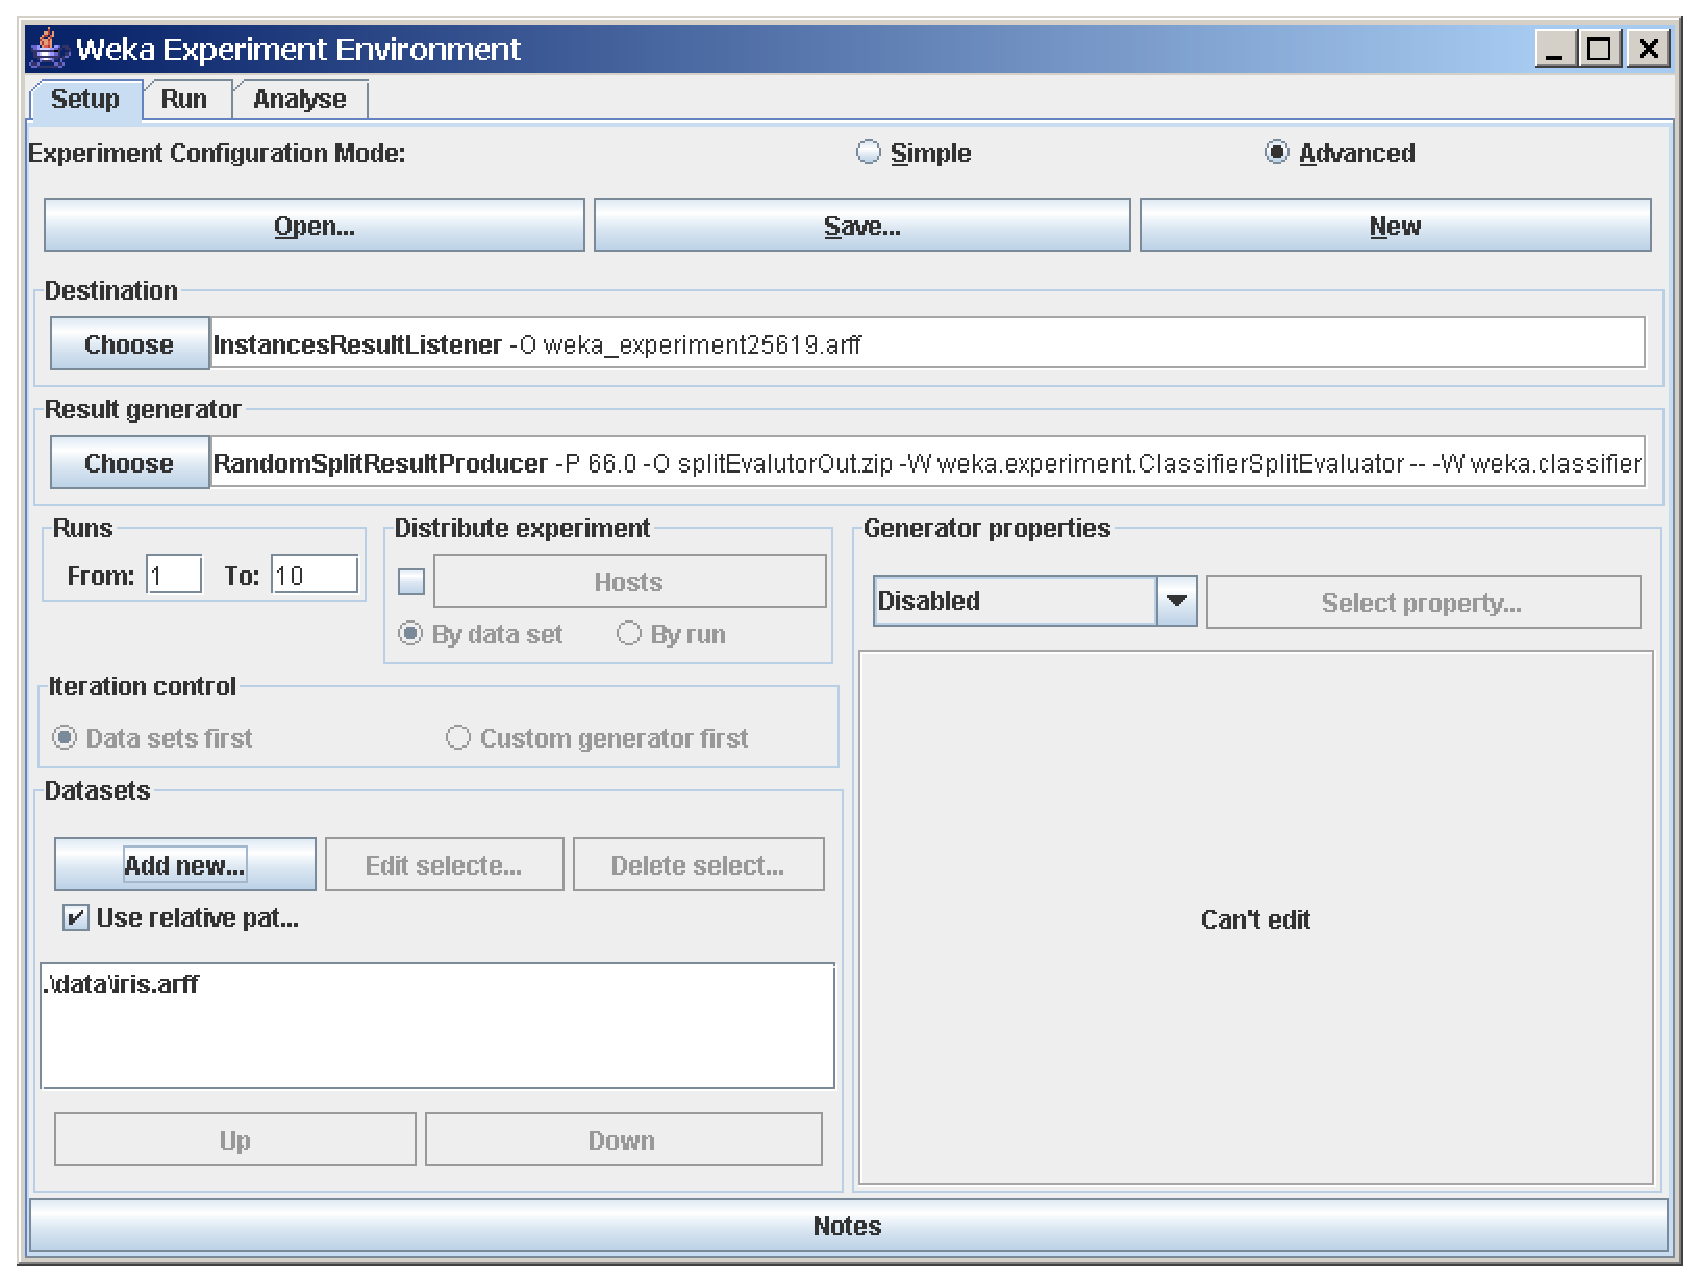
\epsfig{file=images/advanced_adddataset3.eps,width=10cm}
\end{center}

The dataset name is now displayed in the \textit{Datasets} panel of the \textit{Setup} tab.



\subsubsection*{Saving the Results of the Experiment}

To identify a dataset to which the results are to be sent, click on the \textit{InstancesResultListener} entry in the \textit{Destination} panel. The output file parameter is near the bottom of the window, beside the text \textit{outputFile}. Click on this parameter to display a file selection window.
\begin{center}
	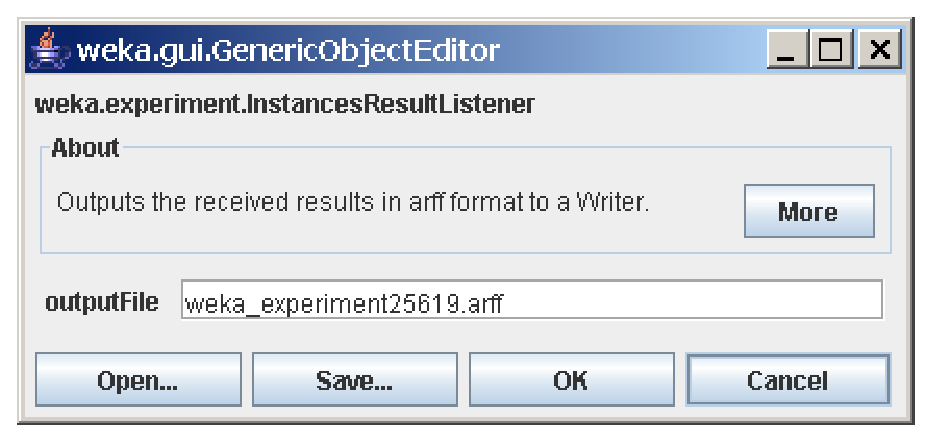
\epsfig{file=images/advanced_saveoutput1.eps,width=6cm}
\end{center}
	
\begin{center}
	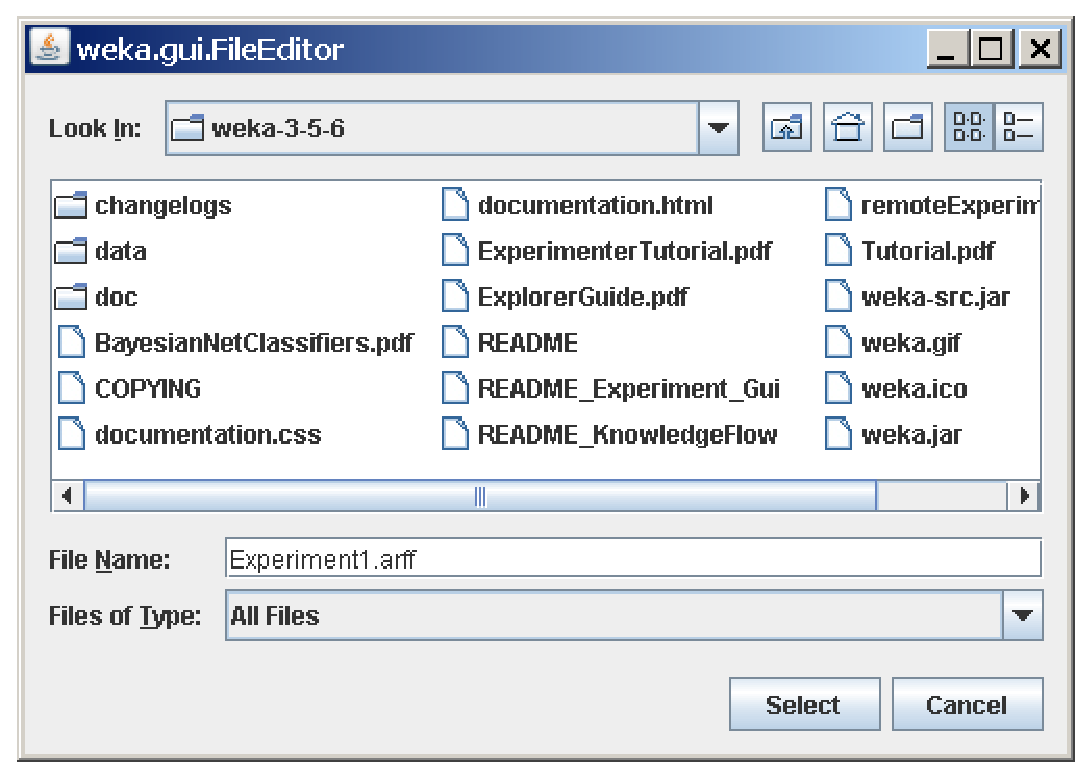
\epsfig{file=images/advanced_saveoutput2.eps,width=7cm}
\end{center}

Type the name of the output file, click \textit{Select}, and then click close (x). The file name is displayed in the \textit{outputFile} panel. Click on \textit{OK} to close the window.
\begin{center}
	\epsfig{file=images/advanced_saveoutput3.eps,width=6cm}
\end{center}

The dataset name is displayed in the \textit{Destination} panel of the \textit{Setup} tab.
\begin{center}
	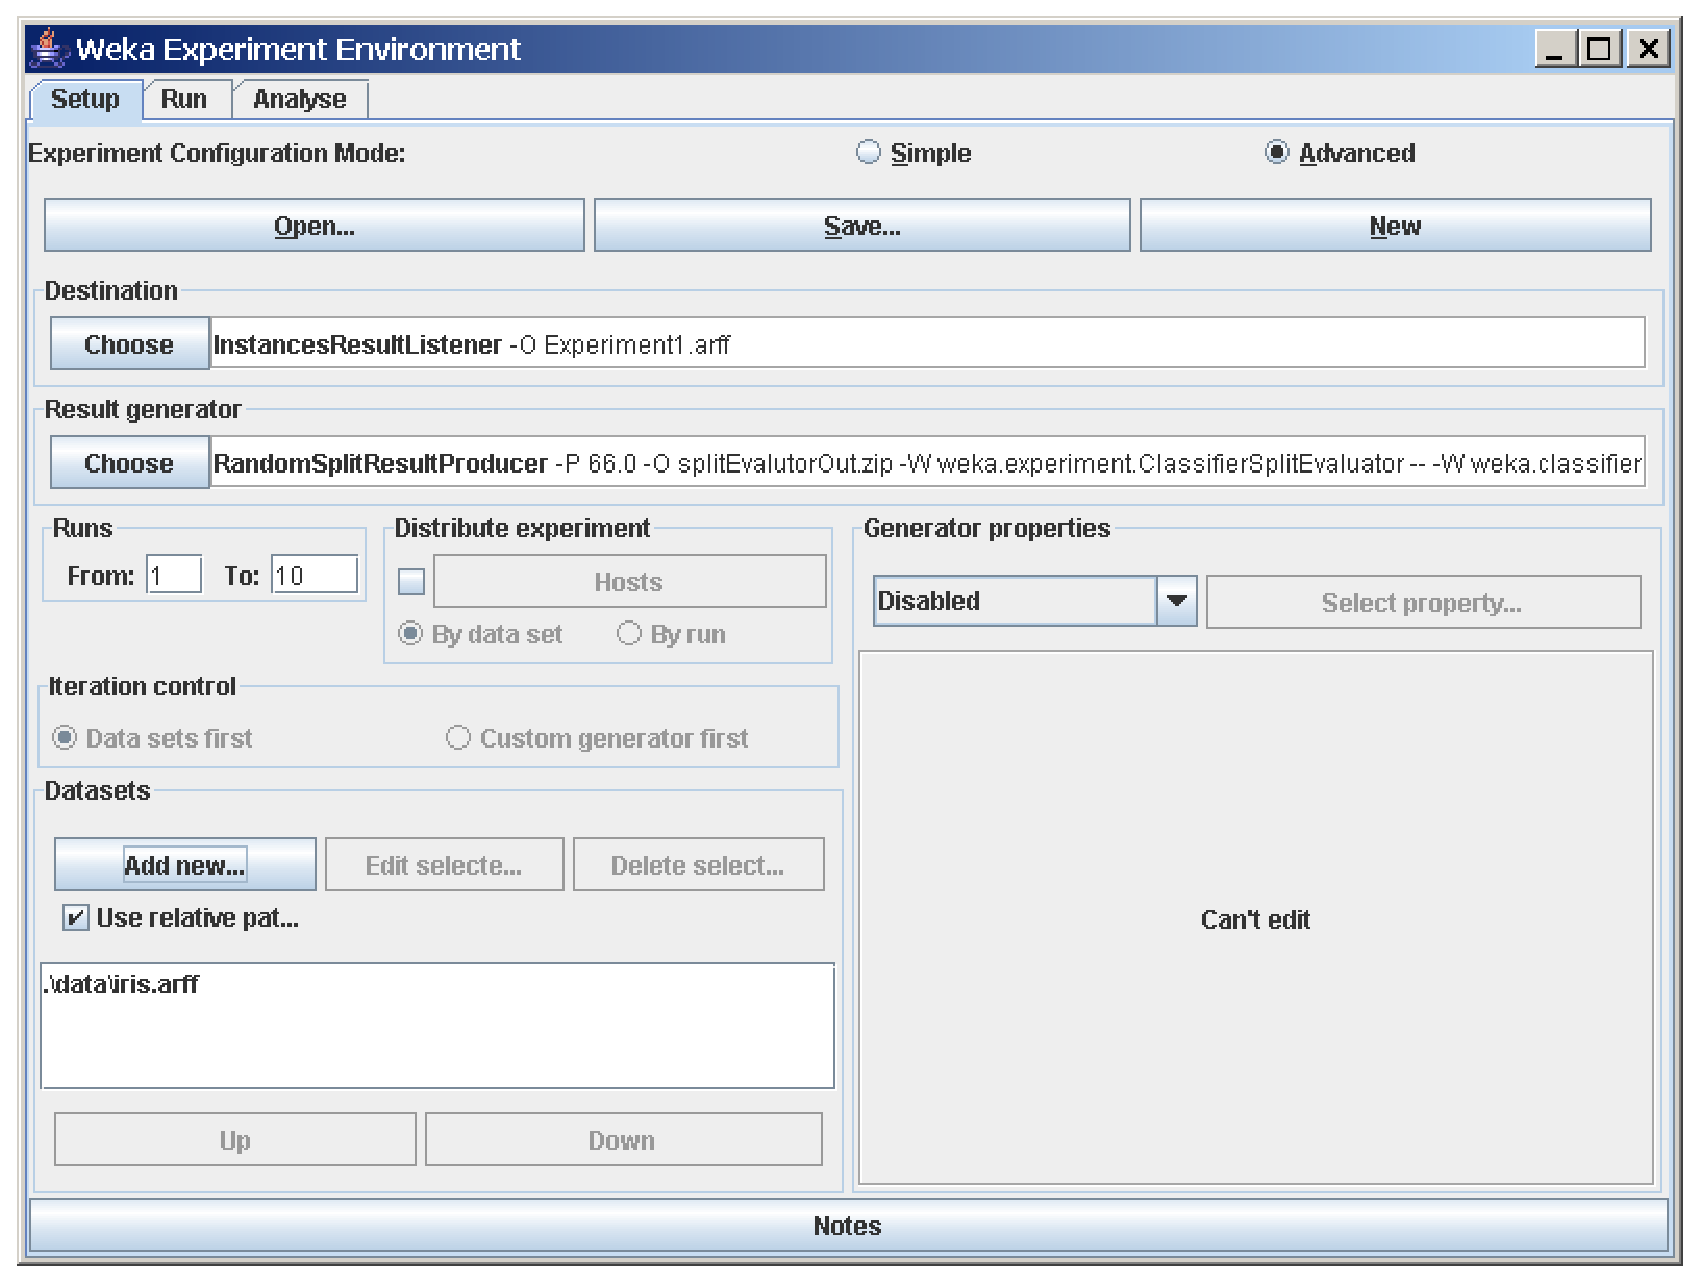
\epsfig{file=images/advanced_saveoutput4.eps,width=10cm}
\end{center}



\subsubsection*{Saving the Experiment Definition}

The experiment definition can be saved at any time. Select \textit{Save...} at the top of the \textit{Setup} tab. Type the dataset name with the extension \textit{exp} (or select the dataset name if the experiment definition dataset already exists) for binary files or choose \textit{Experiment configuration files (*.xml)} from the file types combobox (the XML files are robust with respect to version changes).
\begin{center}
	\epsfig{file=images/advanced_save.eps,width=7cm}
\end{center}


The experiment can be restored by selecting \textit{Open} in the \textit{Setup} tab and then selecting \textit{Experiment1.exp} in the dialog window.



\subsubsection{Running an Experiment}

To run the current experiment, click the \textit{Run} tab at the top of the Experiment Environment window. The current experiment performs 10 randomized train and test runs on the Iris dataset, using 66\% of the patterns for training and 34\% for testing, and using the \texttt{ZeroR} scheme.
\begin{center}
	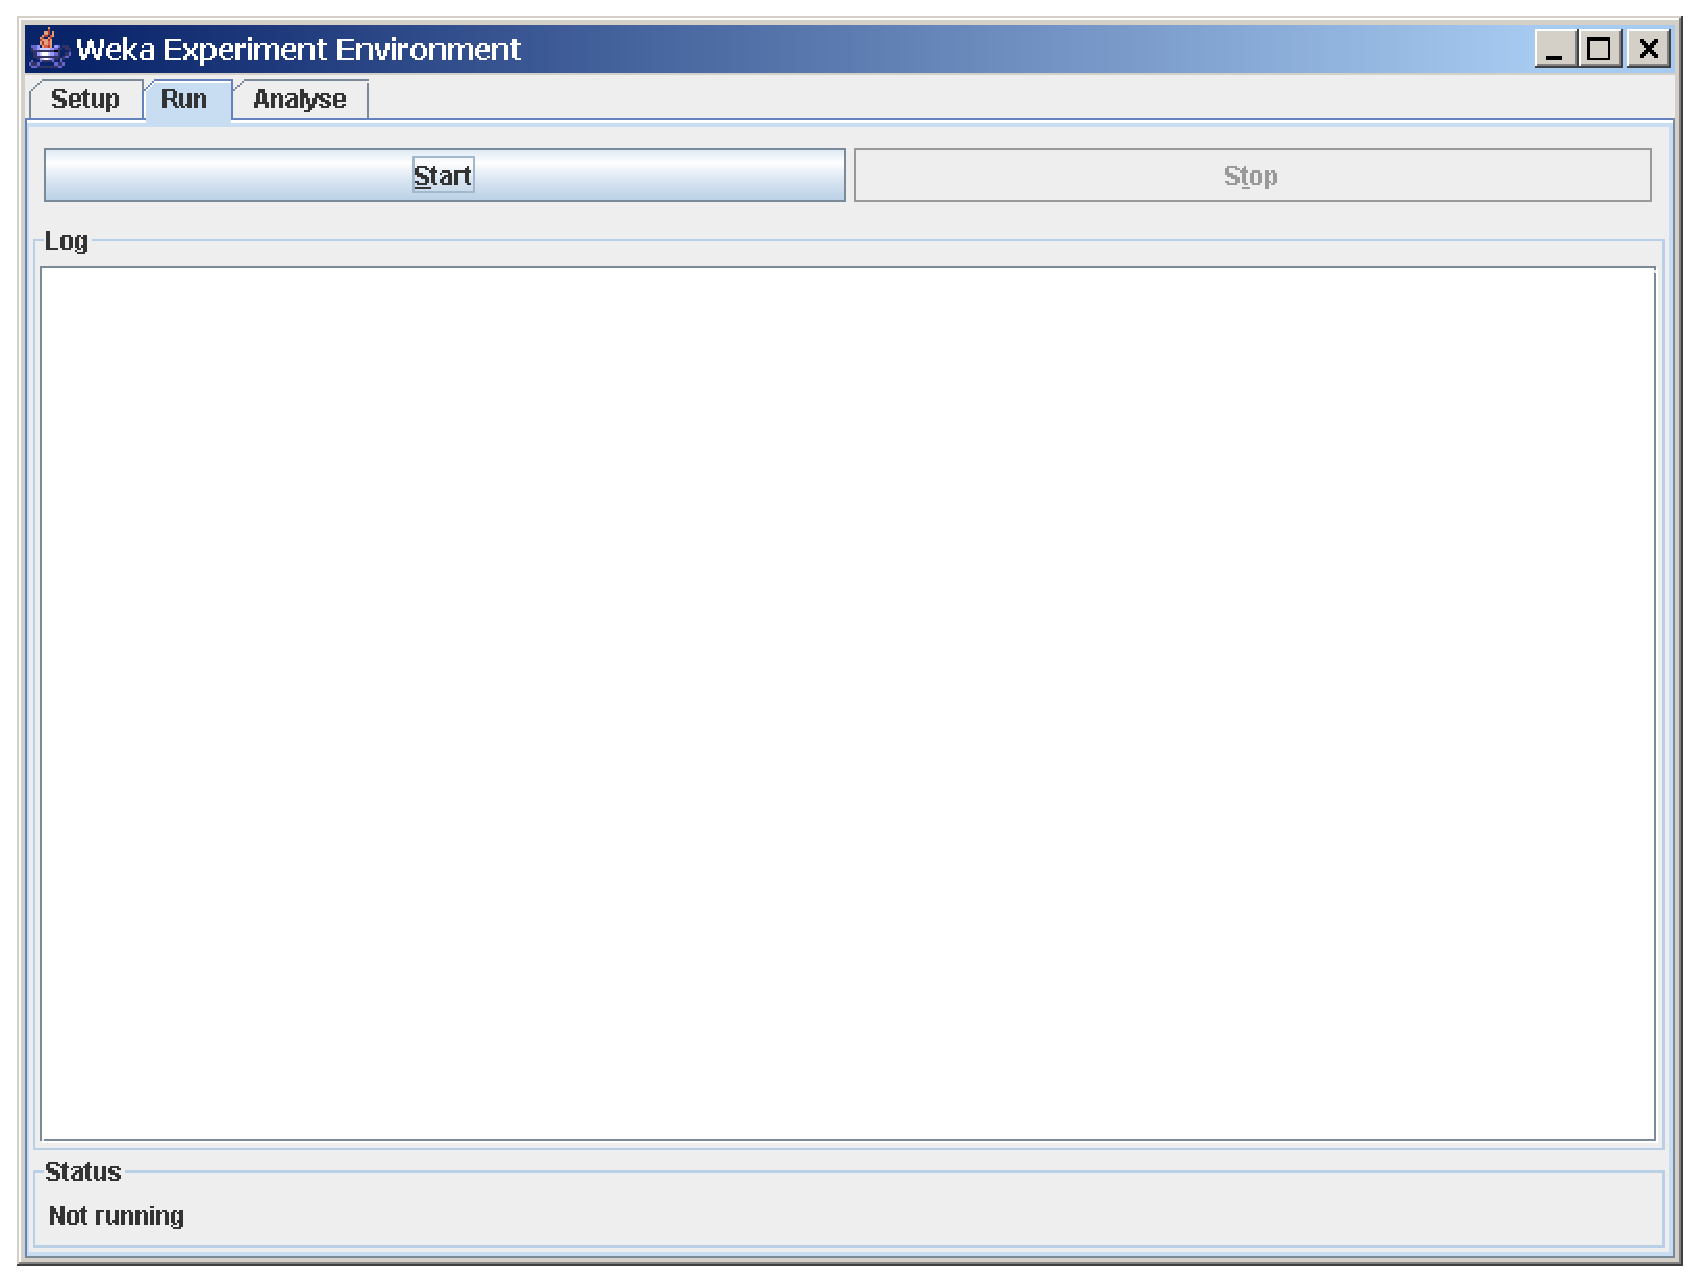
\epsfig{file=images/runexperiment1.eps,width=10cm}
\end{center}

Click \textit{Start} to run the experiment.
\begin{center}
	\epsfig{file=images/runexperiment2.eps,width=10cm}
\end{center}

If the experiment was defined correctly, the 3 messages shown above will be displayed in the \textit{Log} panel. The results of the experiment are saved to the dataset \textit{Experiment1.arff}. The first few lines in this dataset are shown below.

\begin{verbatim}
 @relation InstanceResultListener
 
 @attribute Key_Dataset {iris}
 @attribute Key_Run {1,2,3,4,5,6,7,8,9,10}
 @attribute Key_Scheme {weka.classifiers.rules.ZeroR,weka.classifiers.trees.J48}
 @attribute Key_Scheme_options {,'-C 0.25 -M 2'}
 @attribute Key_Scheme_version_ID {48055541465867954,-217733168393644444}
 @attribute Date_time numeric
 @attribute Number_of_training_instances numeric
 @attribute Number_of_testing_instances numeric
 @attribute Number_correct numeric
 @attribute Number_incorrect numeric
 @attribute Number_unclassified numeric
 @attribute Percent_correct numeric
 @attribute Percent_incorrect numeric
 @attribute Percent_unclassified numeric
 @attribute Kappa_statistic numeric
 @attribute Mean_absolute_error numeric
 @attribute Root_mean_squared_error numeric
 @attribute Relative_absolute_error numeric
 @attribute Root_relative_squared_error numeric
 @attribute SF_prior_entropy numeric
 @attribute SF_scheme_entropy numeric
 @attribute SF_entropy_gain numeric
 @attribute SF_mean_prior_entropy numeric
 @attribute SF_mean_scheme_entropy numeric
 @attribute SF_mean_entropy_gain numeric
 @attribute KB_information numeric
 @attribute KB_mean_information numeric
 @attribute KB_relative_information numeric
 @attribute True_positive_rate numeric
 @attribute Num_true_positives numeric
 @attribute False_positive_rate numeric
 @attribute Num_false_positives numeric
 @attribute True_negative_rate numeric
 @attribute Num_true_negatives numeric
 @attribute False_negative_rate numeric
 @attribute Num_false_negatives numeric
 @attribute IR_precision numeric
 @attribute IR_recall numeric
 @attribute F_measure numeric
 @attribute Area_under_ROC numeric
 @attribute Time_training numeric
 @attribute Time_testing numeric
 @attribute Summary {'Number of leaves: 3\nSize of the tree: 5\n',
    'Number of leaves: 5\nSize of the tree: 9\n',
    'Number of leaves: 4\nSize of the tree: 7\n'}
 @attribute measureTreeSize numeric
 @attribute measureNumLeaves numeric
 @attribute measureNumRules numeric

 @data
 
 iris,1,weka.classifiers.rules.ZeroR,,48055541465867954,20051221.033,99,51,
 17,34,0,33.333333,66.666667,0,0,0.444444,0.471405,100,100,80.833088,80.833088,
 0,1.584963,1.584963,0,0,0,0,1,17,1,34,0,0,0,0,0.333333,1,0.5,0.5,0,0,?,?,?,?
\end{verbatim}




\subsubsection{Changing the Experiment Parameters}

\subsubsection*{Changing the Classifier}

The parameters of an experiment can be changed by clicking on the \textit{Result generator} panel.
\begin{center}
	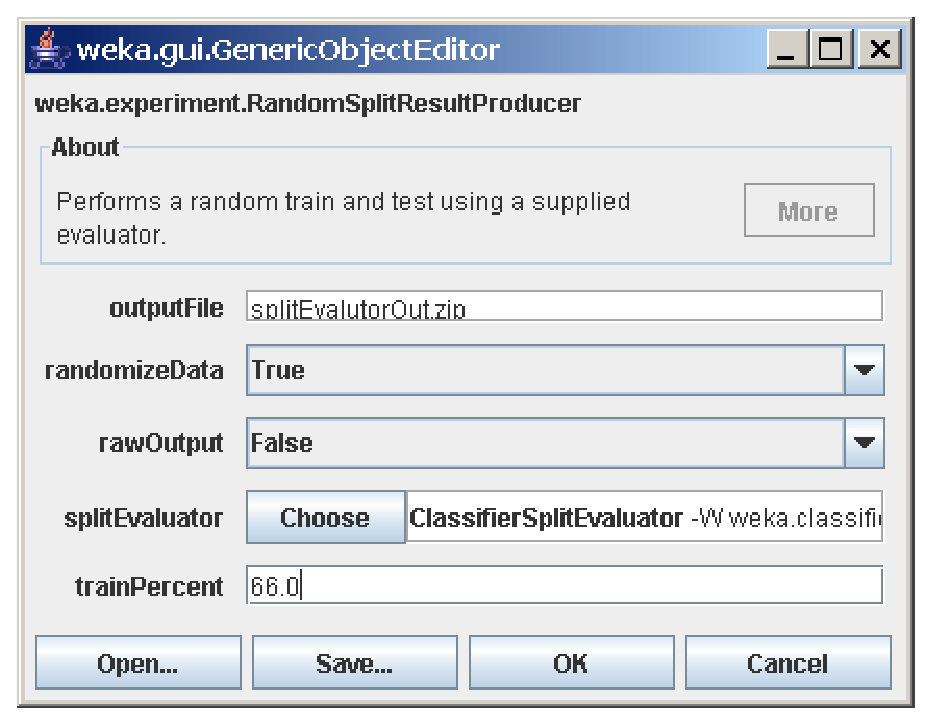
\epsfig{file=images/advanced_changeparameters1.eps,width=6cm}
\end{center}

The \textit{RandomSplitResultProducer} performs repeated train/test runs. The number of instances (expressed as a percentage) used for training is given in the \textit{trainPercent} box. (The number of runs is specified in the \textit{Runs} panel in the \textit{Setup} tab.)

A small help file can be displayed by clicking \textit{More} in the \textit{About} panel.
\begin{center}
	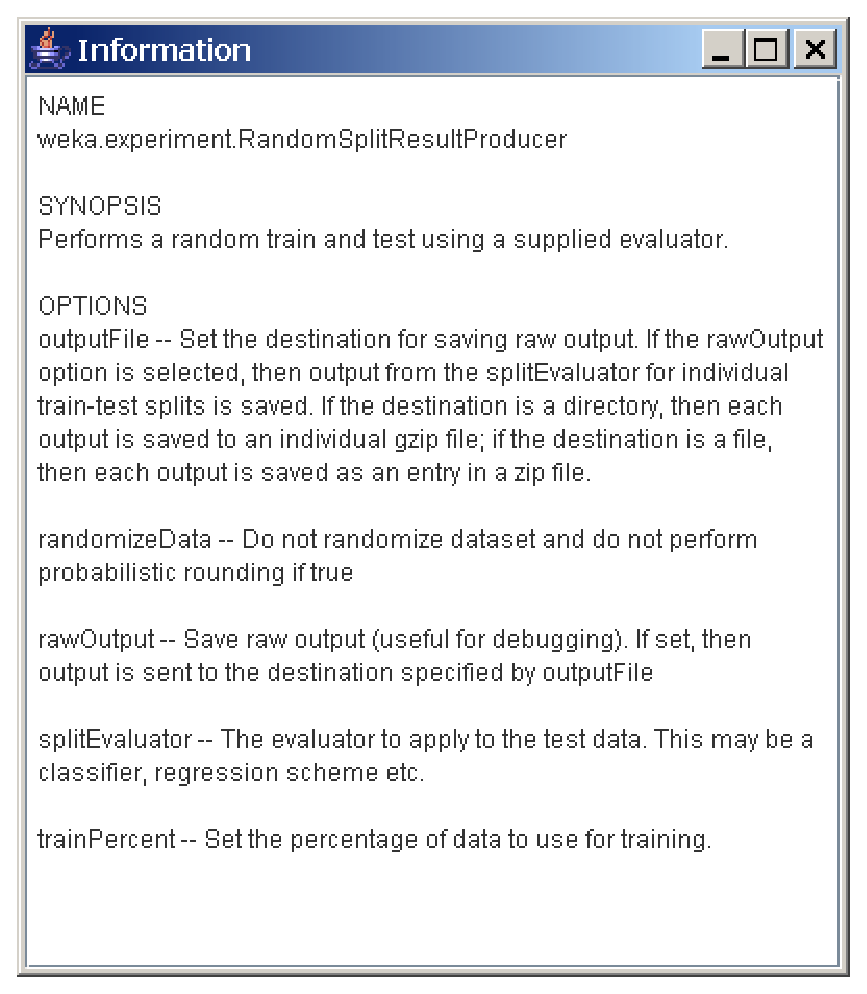
\epsfig{file=images/advanced_changeparameters2.eps,width=6cm}
\end{center}

Click on the \textit{splitEvaluator} entry to display the \textit{SplitEvaluator} properties.
\begin{center}
	\epsfig{file=images/advanced_changeparameters3.eps,width=6cm}
\end{center}

Click on the classifier entry (\texttt{ZeroR}) to display the scheme properties.
\begin{center}
	\epsfig{file=images/advanced_changeparameters4.eps,width=6cm}
\end{center}

This scheme has no modifiable properties (besides \textit{debug} mode on/off) but most other schemes do have properties that can be modified by the user. The \textit{Capabilities} button opens a small dialog listing all the attribute and class types this classifier can handle. Click on the \textit{Choose} button to select a different scheme. The window below shows the parameters available for the \texttt{J48} decision-tree scheme. If desired, modify the parameters and then click \textit{OK} to close the window.
\begin{center}
	\epsfig{file=images/advanced_changeparameters5.eps,width=6cm}
\end{center}

The name of the new scheme is displayed in the \textit{Result generator} panel.
\begin{center}
	\epsfig{file=images/advanced_changeparameters6.eps,width=10cm}
\end{center}


\subsubsection*{Adding Additional Schemes}

Additional schemes can be added in the \textit{Generator properties} panel. To begin, change the drop-down list entry from \textit{Disabled} to \textit{Enabled} in the \textit{Generator properties} panel.
\begin{center}
	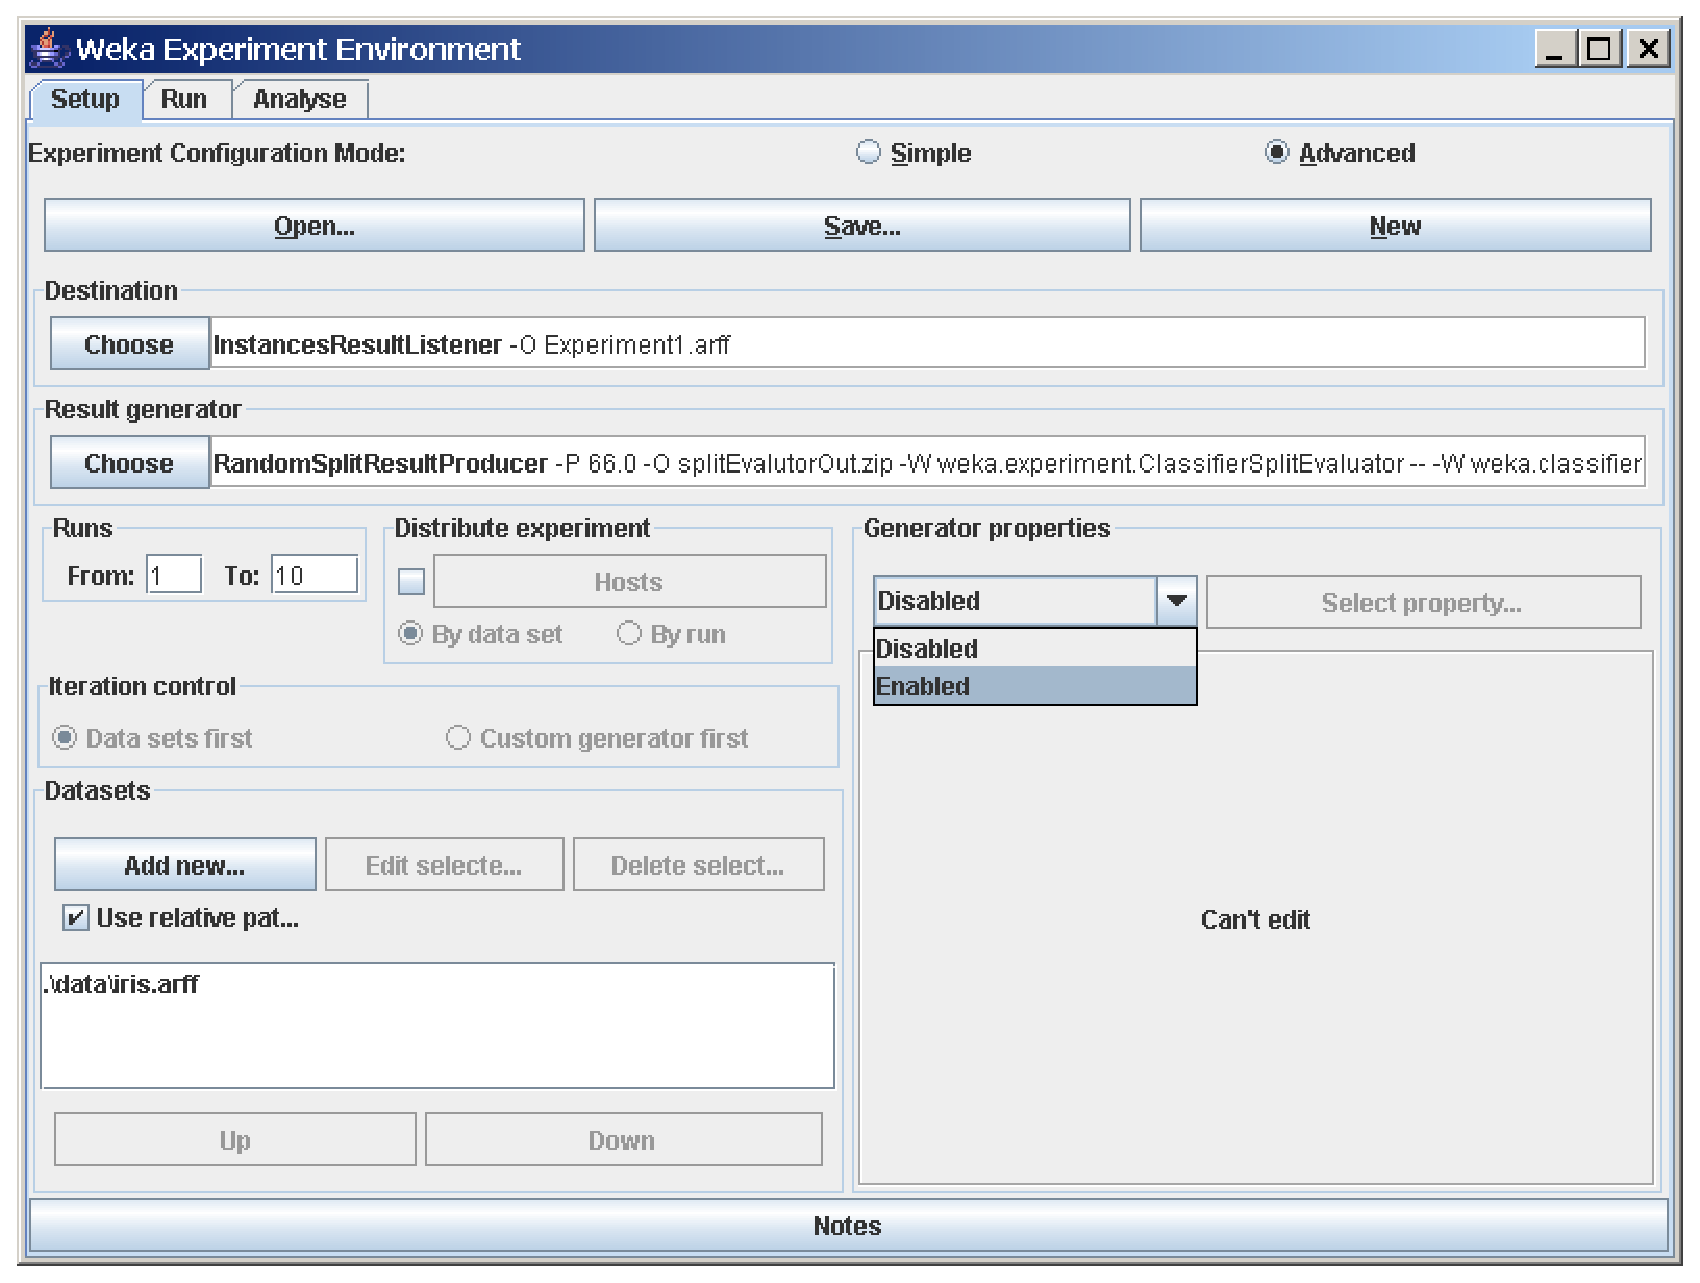
\epsfig{file=images/advanced_additionalschemes1.eps,width=10cm}
\end{center}

Click \textit{Select property} and expand \textit{splitEvaluator} so that the \textit{classifier} entry is visible in the property list; click \textit{Select}.
\begin{center}
	\epsfig{file=images/advanced_additionalschemes2.eps,width=3.5cm}
\end{center}

The scheme name is displayed in the \textit{Generator properties} panel.
\begin{center}
	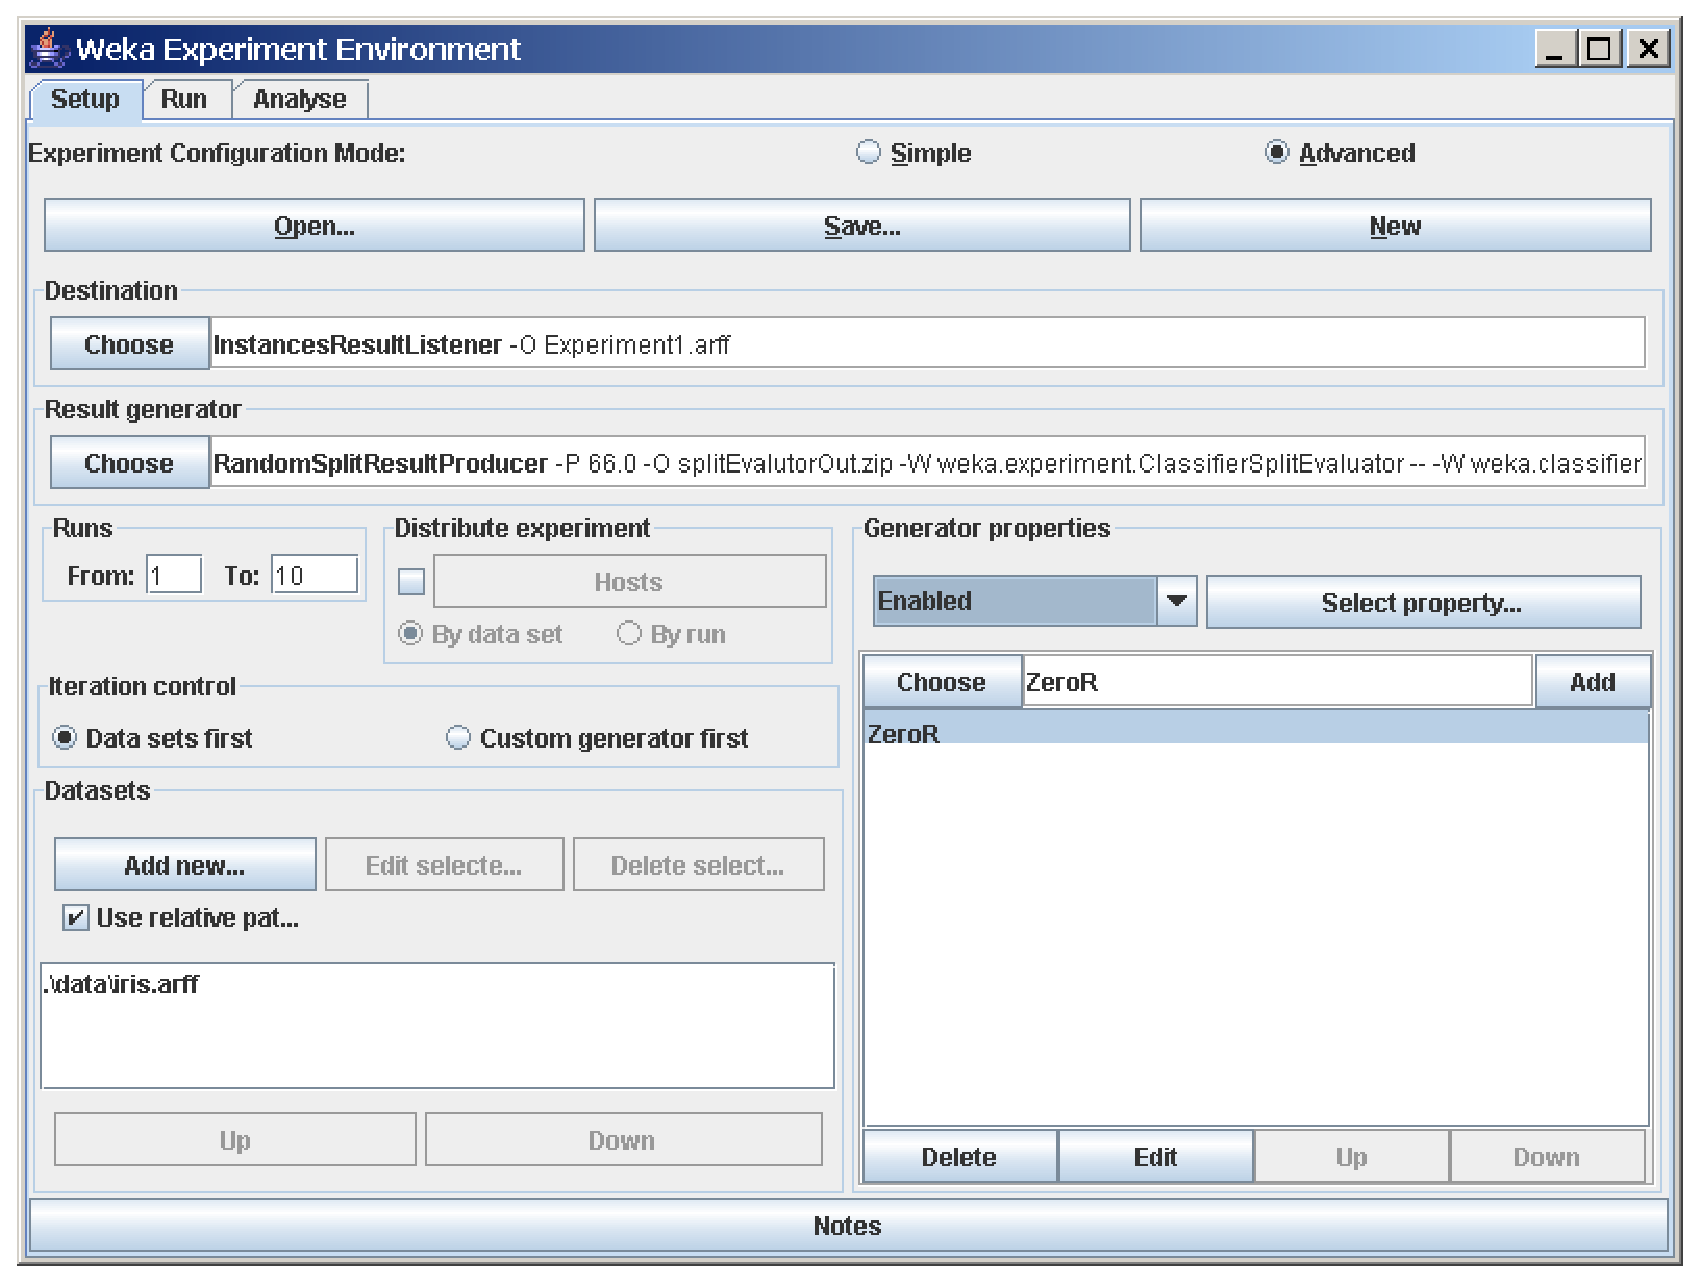
\epsfig{file=images/advanced_additionalschemes3.eps,width=10cm}
\end{center}

To add another scheme, click on the \textit{Choose} button to display the \textit{GenericObjectEditor} window.
\begin{center}
	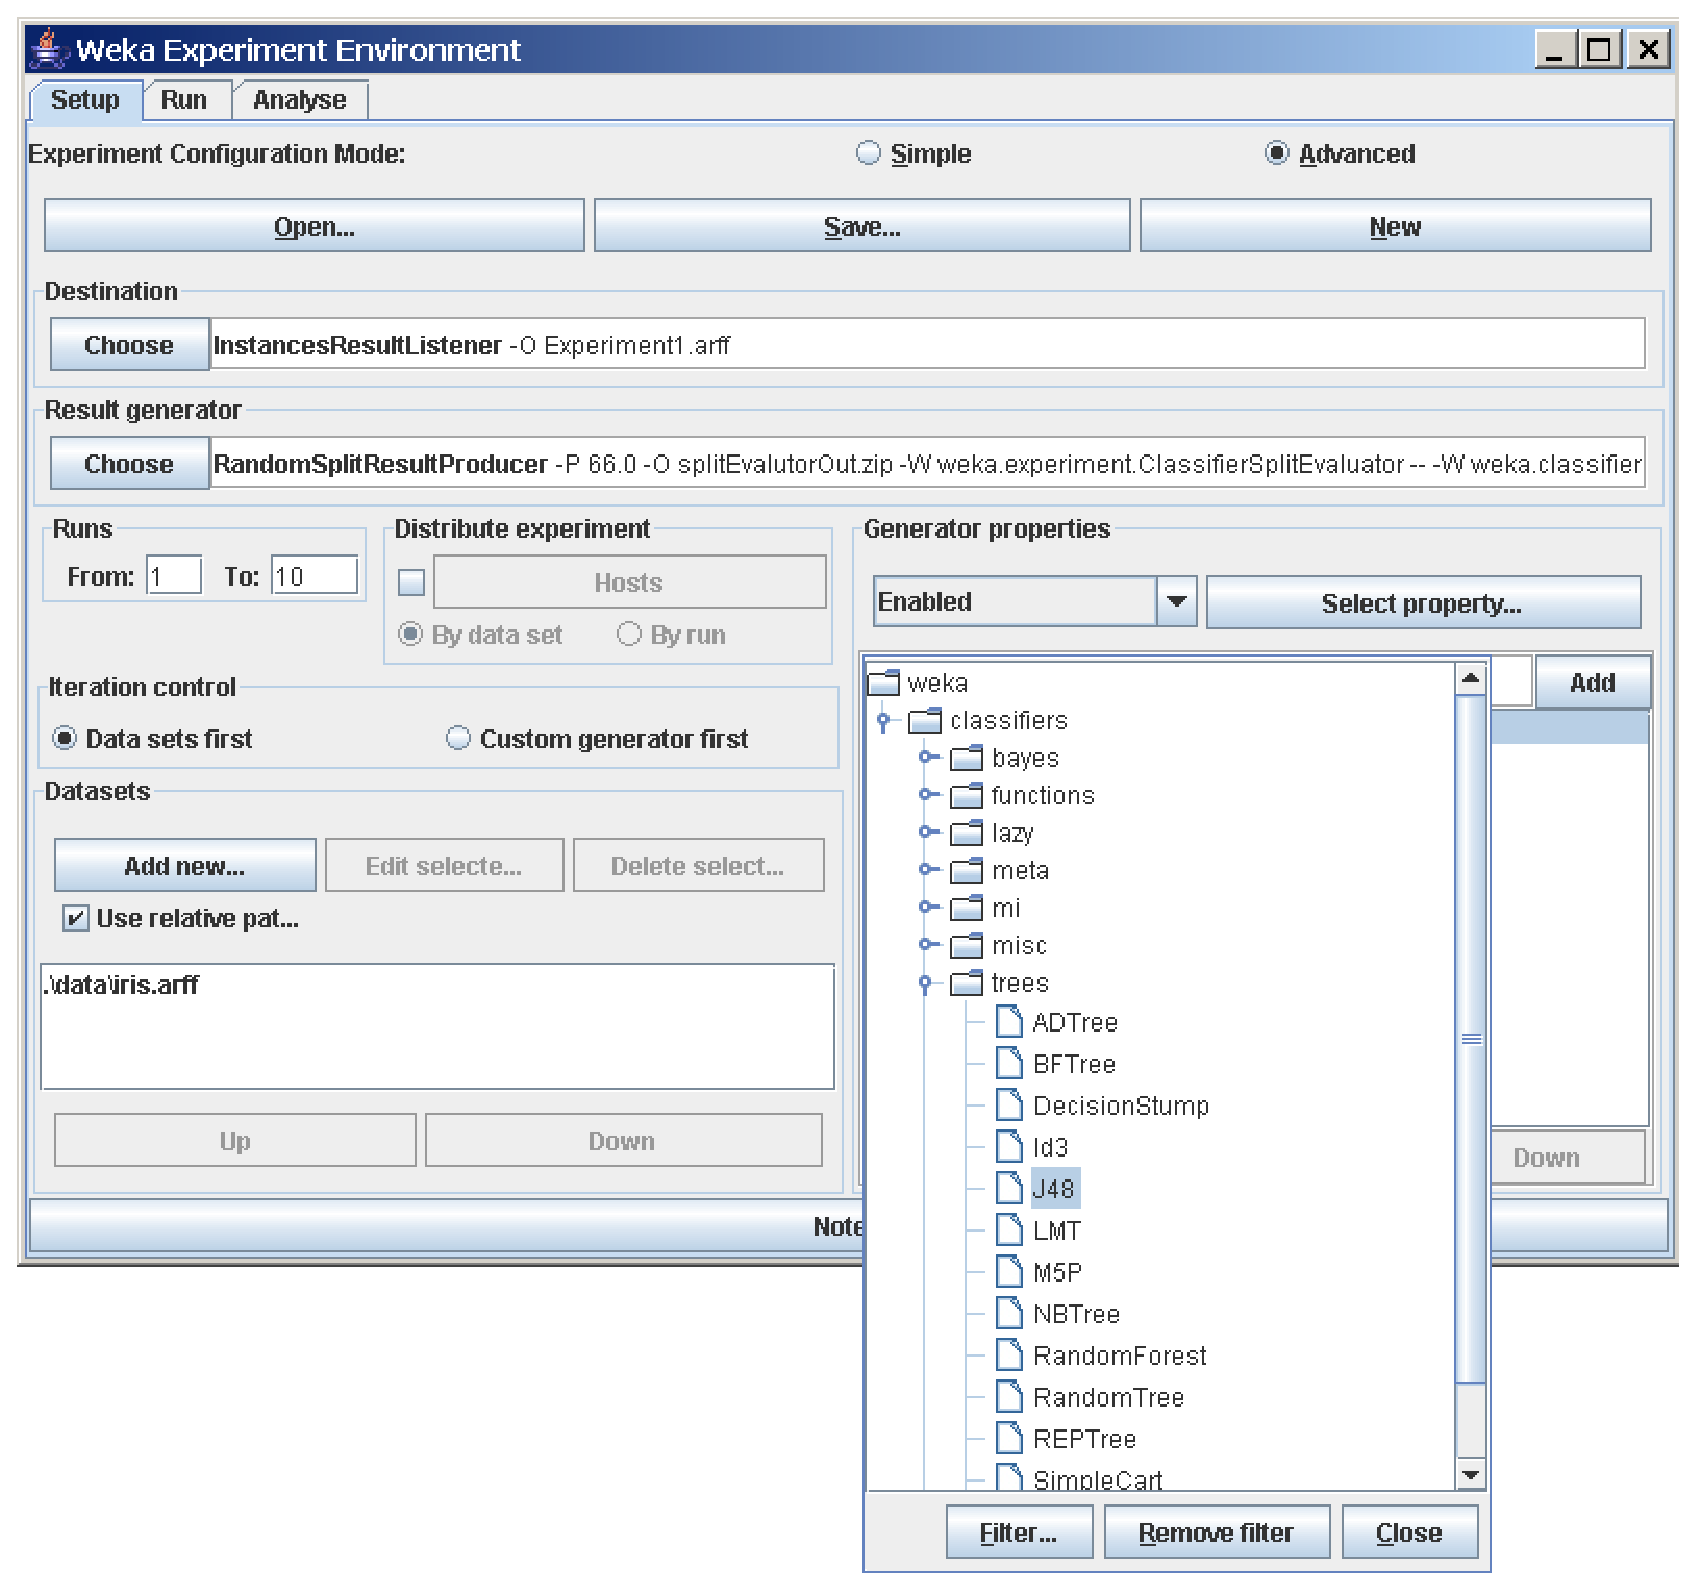
\epsfig{file=images/advanced_additionalschemes4.eps,width=10cm}
\end{center}

The \textit{Filter...} button enables one to highlight classifiers that can handle certain attribute and class types. With the \textit{Remove filter} button all the selected capabilities will get cleared and the highlighting removed again.

To change to a decision-tree scheme, select \texttt{J48} (in subgroup \textit{trees}).
\begin{center}
	\epsfig{file=images/advanced_additionalschemes5.eps,width=6cm}
\end{center}

The new scheme is added to the \textit{Generator properties} panel. Click \textit{Add} to add the new scheme.
\begin{center}
	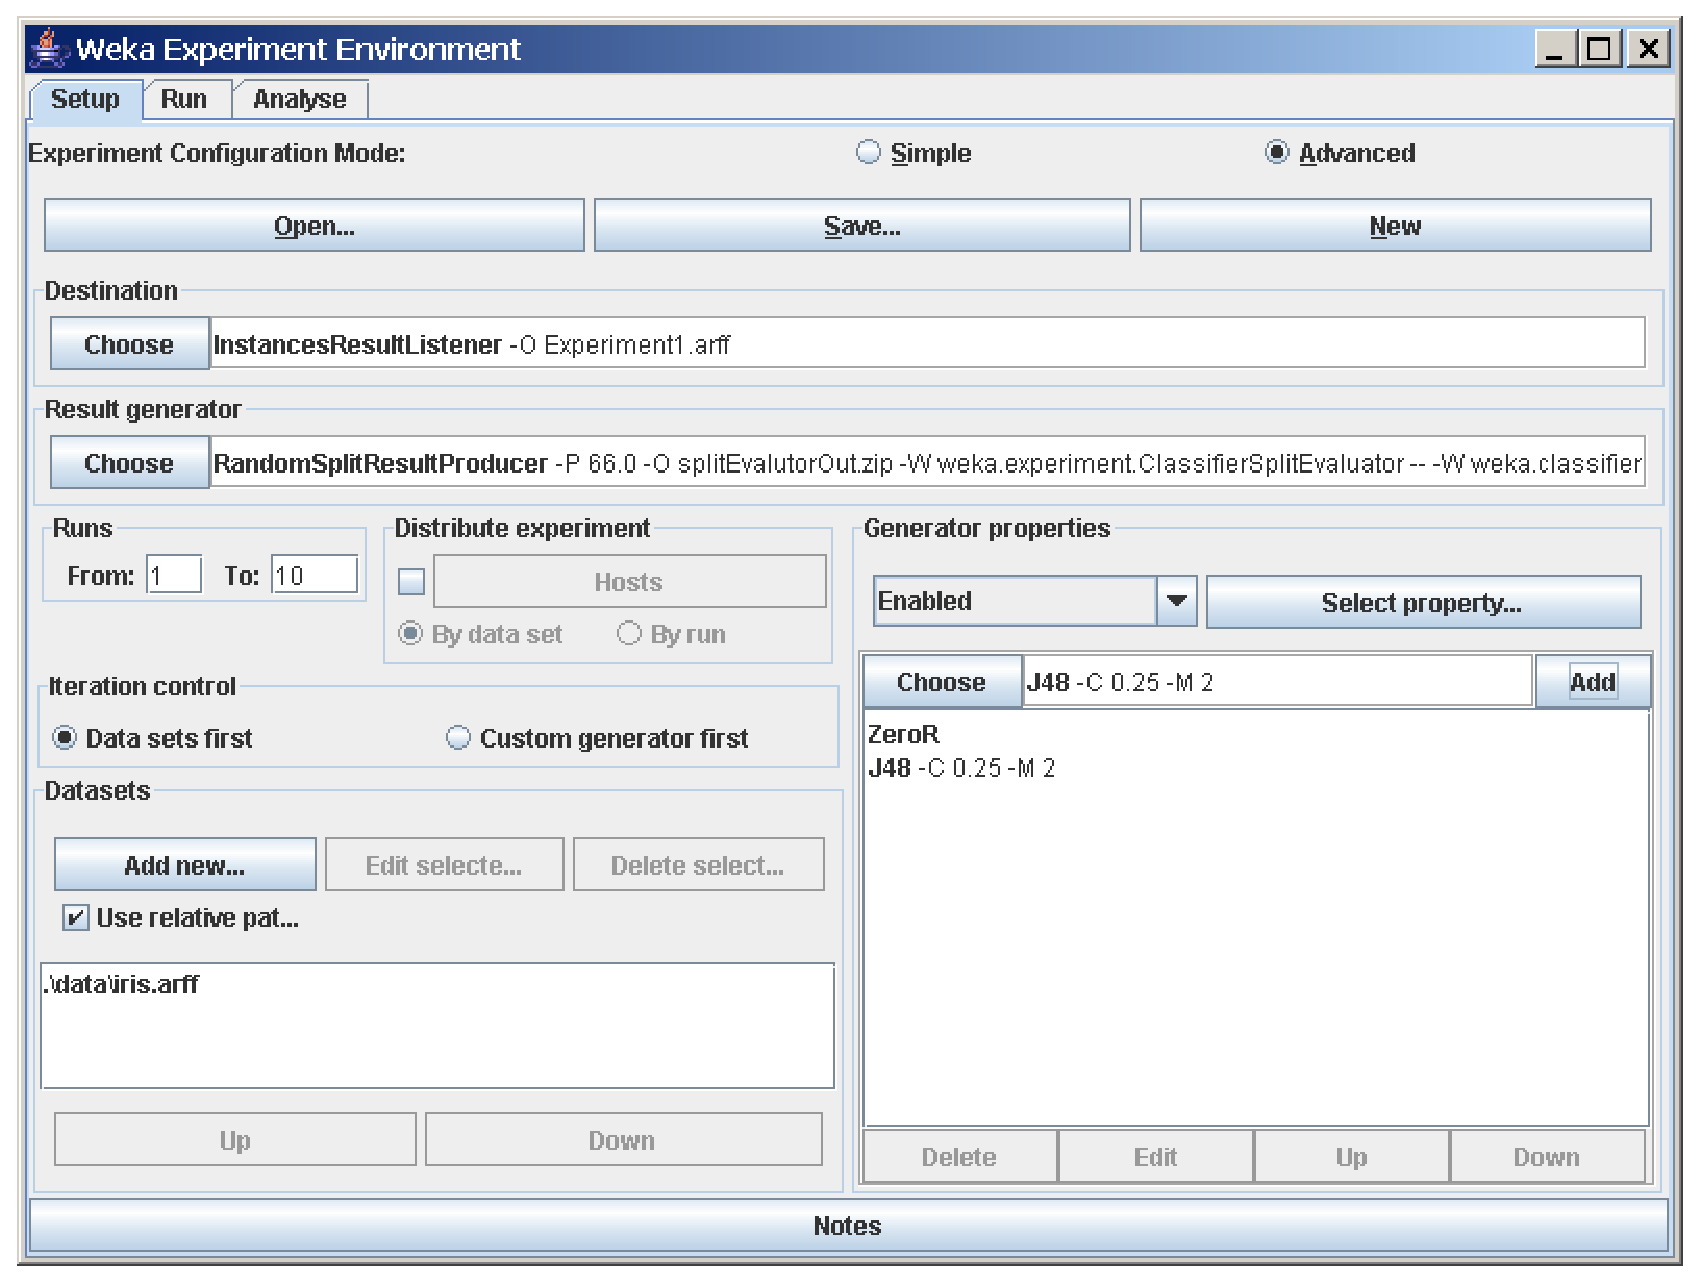
\epsfig{file=images/advanced_additionalschemes6.eps,width=10cm}
\end{center}

Now when the experiment is run, results are generated for both schemes.

To add additional schemes, repeat this process. To remove a scheme, select the scheme by clicking on it and then click \textit{Delete}.


\subsubsection*{Adding Additional Datasets}

The scheme(s) may be run on any number of datasets at a time. Additional datasets are added by clicking \textit{Add new...} in the \textit{Datasets} panel. Datasets are deleted from the experiment by selecting the dataset and then clicking \textit{Delete Selected}.


\subsubsection*{Raw Output}

The raw output generated by a scheme during an experiment can be saved to a file and then examined at a later time. Open the \textit{ResultProducer} window by clicking on the \textit{Result generator} panel in the \textit{Setup} tab.
\begin{center}
	\epsfig{file=images/advanced_rawoutput1.eps,width=6cm}
\end{center}

Click on \textit{rawOutput} and select the \textit{True} entry from the drop-down list. By default, the output is sent to the zip file \textit{splitEvaluatorOut.zip}. The output file can be changed by clicking on the \textit{outputFile} panel in the window. Now when the experiment is run, the result of each processing run is archived, as shown below.
\begin{center}
	\epsfig{file=images/advanced_rawoutput2.eps,width=10cm}
\end{center}

The contents of the first run are:

\begin{verbatim}
ClassifierSplitEvaluator: weka.classifiers.trees.J48 -C 0.25 -M 2(version 
     -217733168393644444)Classifier model: 
J48 pruned tree
------------------

petalwidth <= 0.6: Iris-setosa (33.0)
petalwidth > 0.6
|   petalwidth <= 1.5: Iris-versicolor (31.0/1.0)
|   petalwidth > 1.5: Iris-virginica (35.0/3.0) 

Number of Leaves  : 	3

Size of the tree : 	5 


Correctly Classified Instances          47               92.1569 %
Incorrectly Classified Instances         4                7.8431 %
Kappa statistic                          0.8824
Mean absolute error                      0.0723
Root mean squared error                  0.2191
Relative absolute error                 16.2754 %
Root relative squared error             46.4676 %
Total Number of Instances               51     
measureTreeSize : 5.0
measureNumLeaves : 3.0
measureNumRules : 3.0
\end{verbatim}



\subsubsection{Other Result Producers}

\subsubsection*{Cross-Validation Result Producer}

To change from random train and test experiments to cross-validation experiments, click on the \textit{Result generator} entry. At the top of the window, click on the drop-down list and select \textit{CrossValidationResultProducer}. The window now contains parameters specific to cross-validation such as the number of partitions/folds. The experiment performs 10-fold cross-validation instead of train and test in the given example.
\begin{center}
	\epsfig{file=images/advanced_cvresultproducer1.eps,width=6cm}
\end{center}

The \textit{Result generator} panel now indicates that cross-validation will be performed. Click on \textit{More} to generate a brief description of the \textit{CrossValidationResultProducer}.
\begin{center}
	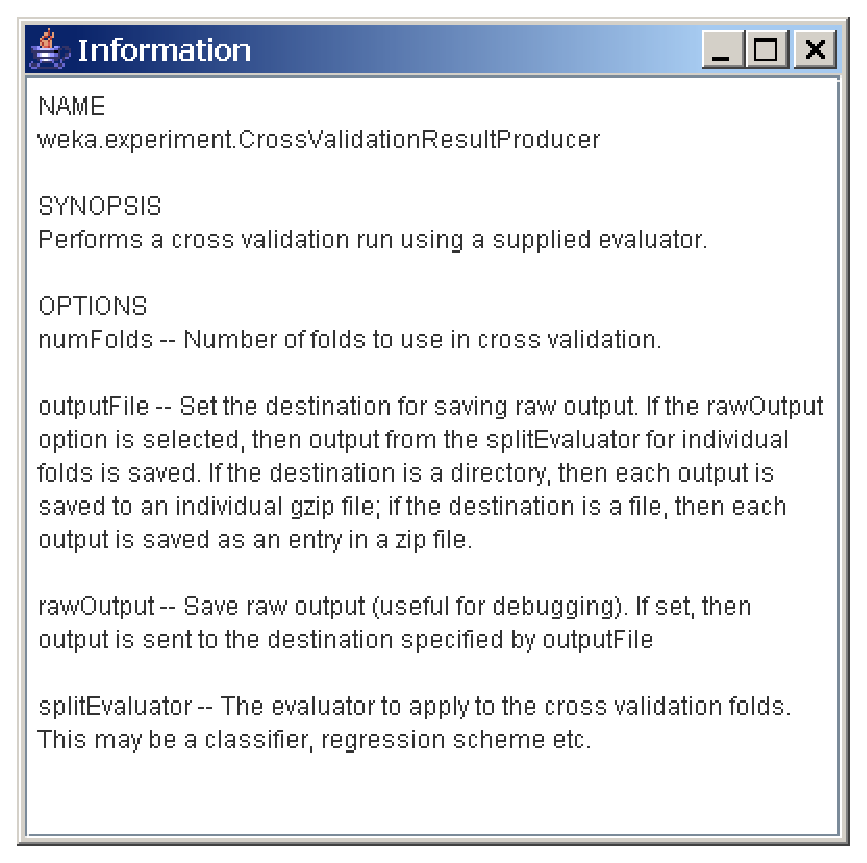
\epsfig{file=images/advanced_cvresultproducer2.eps,width=6cm}
\end{center}

As with the \textit{RandomSplitResultProducer}, multiple schemes can be run during cross-validation by adding them to the \textit{Generator properties} panel.
\begin{center}
	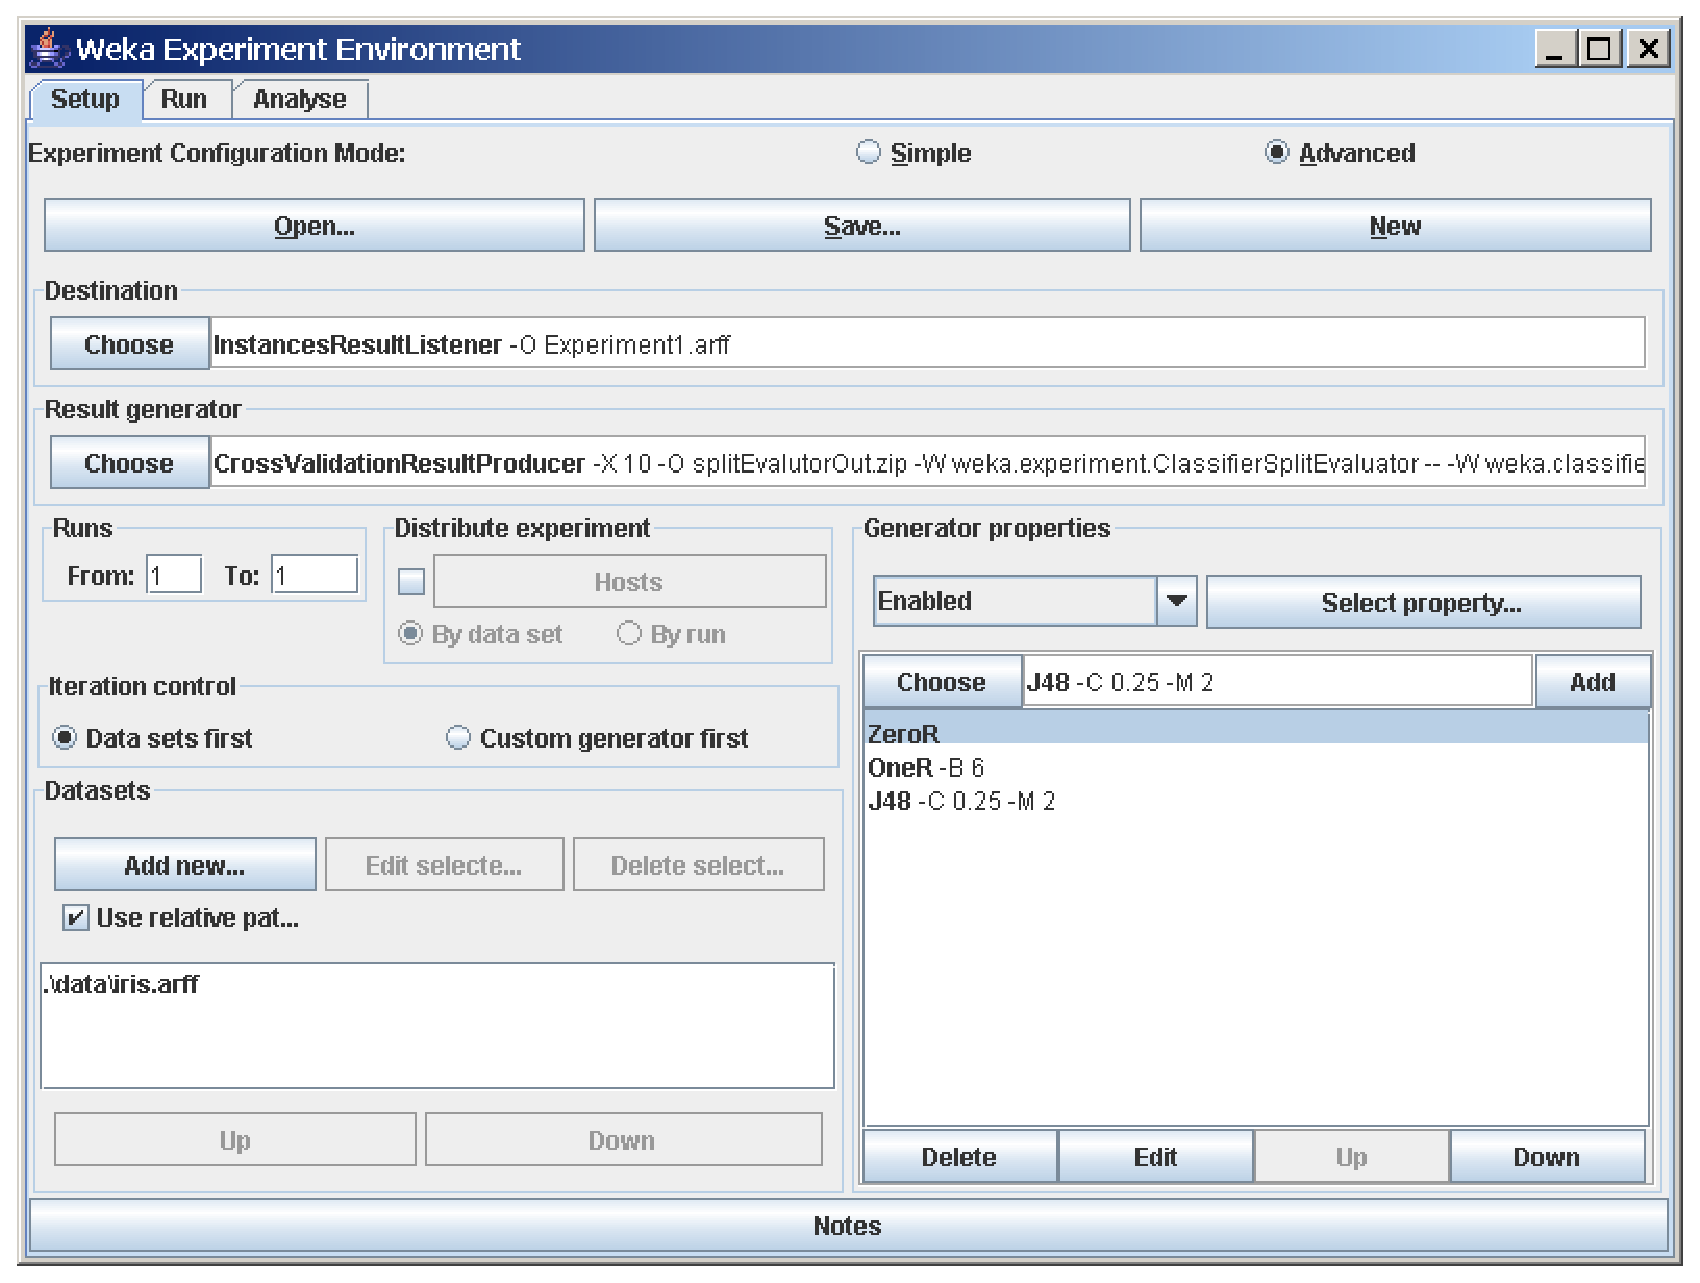
\epsfig{file=images/advanced_cvresultproducer3.eps,width=10cm}
\end{center}

The number of runs is set to 1 in the \textit{Setup} tab in this example, so that only one run of cross-validation for each scheme and dataset is executed.

When this experiment is analysed, the following results are generated. Note that there are 30 (1 run times 10 folds times 3 schemes) result lines processed.
\begin{center}
	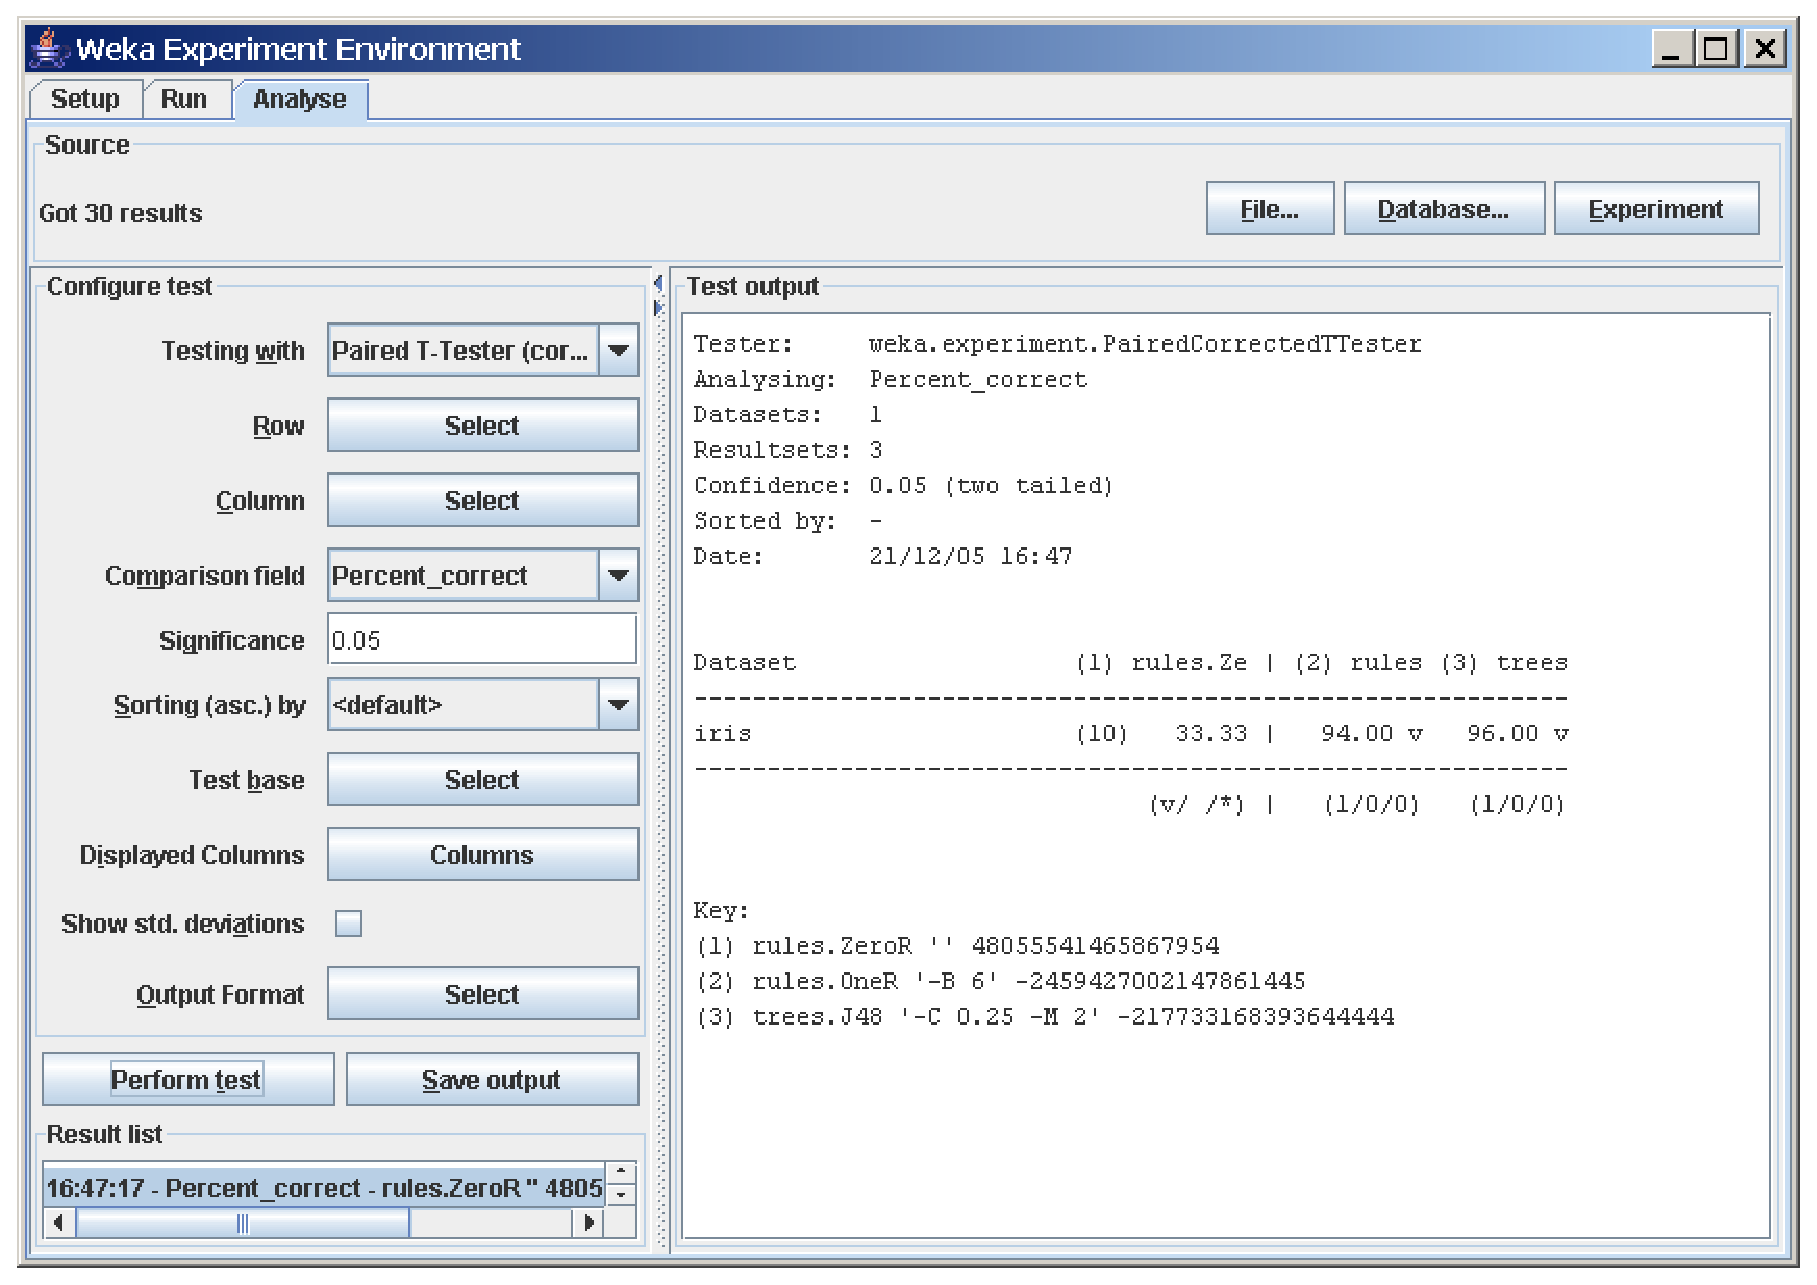
\epsfig{file=images/advanced_cvresultproducer4.eps,width=10cm}
\end{center}


\subsubsection*{Averaging Result Producer}

An alternative to the \textit{CrossValidationResultProducer} is the \textit{AveragingResultProducer}. This result producer takes the average of a set of runs (which are typically cross-validation runs). This result producer is identified by clicking the \textit{Result generator} panel and then choosing the \textit{AveragingResultProducer} from the \textit{GenericObjectEditor}.
\begin{center}
	\epsfig{file=images/advanced_averagingresultproducer1.eps,width=6cm}
\end{center}

The associated help file is shown below.
\begin{center}
	\epsfig{file=images/advanced_averagingresultproducer2.eps,width=6cm}
\end{center}

Clicking the \textit{resultProducer} panel brings up the following window.
\begin{center}
	\epsfig{file=images/advanced_averagingresultproducer3.eps,width=6cm}
\end{center}

As with the other ResultProducers, additional schemes can be defined. When the \textit{AveragingResultProducer} is used, the classifier property is located deeper in the \textit{Generator properties} hierarchy.
\begin{center}
	\epsfig{file=images/advanced_averagingresultproducer4.eps,width=3.5cm}
\end{center}
	
\begin{center}
	\epsfig{file=images/advanced_averagingresultproducer5.eps,width=10cm}
\end{center}

In this experiment, the \texttt{ZeroR}, \texttt{OneR}, and \texttt{J48} schemes are run 10 times with 10-fold cross-validation. Each set of 10 cross-validation folds is then averaged, producing one result line for each run (instead of one result line for each fold as in the previous example using the \textit{CrossValidationResultProducer}) for a total of 30 result lines. If the raw output is saved, all 300 results are sent to the archive.
\begin{center}
	\epsfig{file=images/advanced_averagingresultproducer6.eps,width=10cm}
\end{center}


%%%%%%%%%%%%%%%%%%%%%%
% Remote Experiments %
%%%%%%%%%%%%%%%%%%%%%%

\newpage
\section{Remote Experiments}

Remote experiments enable you to distribute the computing load across multiple computers. In the following we will discuss the setup and operation for HSQLDB \cite{hsql} and MySQL \cite{mysql}.

\subsection{Preparation}

To run a remote experiment you will need:

\begin{itemize}
   \item A database server.
   \item A number of computers to run remote engines on.
   \item To edit the remote engine policy file included in the Weka distribution to allow Java class and dataset loading from your home directory.
   \item An invocation of the Experimenter on a machine somewhere (any will do).
\end{itemize}

\noindent For the following examples, we assume a user called \textit{johndoe} with this setup:

\begin{itemize}
	\item Access to a set of computers running a flavour of Unix (pathnames need to be changed for Windows).
   \item The home directory is located at \texttt{/home/johndoe}.
   \item Weka is found in \texttt{/home/johndoe/weka}.
   \item Additional jar archives, i.e., JDBC drivers, are stored in \texttt{/home/johndoe/jars}.
   \item The directory for the datasets is \texttt{/home/johndoe/datasets}.
\end{itemize}

\noindent \textbf{Note:} The example policy file \texttt{remote.policy.example} is using this setup (available in \texttt{weka/experiment}\footnote{Weka's source code can be found in the \texttt{weka-src.jar} archive or obtained from CVS \cite{cvs}.}).

\subsection{Database Server Setup}

\begin{itemize}
	\item HSQLDB
	
		\begin{itemize}
			\item Download the JDBC driver for HSQLDB, extract the \texttt{hsqldb.jar} and place it in the directory \texttt{/home/johndoe/jars}.
			
			\item To set up the database server, choose or create a directory to run the database server from, and start the server with:

				\begin{verbatim}
java -classpath /home/johndoe/jars/hsqldb.jar \
  org.hsqldb.Server \
  -database.0 experiment -dbname.0 experiment
				\end{verbatim}
				
				\textbf{Note:} This will start up a database with the alias ``experiment'' (\texttt{-dbname.0 <alias>}) and create a properties and a log file at the current location prefixed with ``experiment'' (\texttt{-database.0 <file>}).
				
		\end{itemize}
		
	\item MySQL
	
We won't go into the details of setting up a MySQL server, but this is rather straightforward and includes the following steps:

		\begin{itemize}
  			\item Download a suitable version of MySQL for your server machine.
  			\item Install and start the MySQL server.
  			\item Create a database - for our example we will use \texttt{experiment} as database name.
  			\item Download the appropriate JDBC driver, extract the JDBC jar and place it as \texttt{mysql.jar} in \texttt{/home/johndoe/jars}.
		\end{itemize}
		
\end{itemize}

\subsection{Remote Engine Setup}

\begin{itemize}
   \item First, set up a directory for scripts and policy files: 
		\begin{verbatim}
/home/johndoe/remote_engine
		\end{verbatim}

   \item Unzip the \texttt{remoteExperimentServer.jar} (from the Weka distribution; or build it from the sources\footnote{Weka's source code can be found in the \texttt{weka-src.jar} archive or obtained from CVS \cite{cvs}.} with \texttt{ant remotejar}) into a temporary directory.

   \item Next, copy \texttt{remoteEngine.jar} and \texttt{remote.policy.example} to the \\ \texttt{/home/johndoe/remote\_engine} directory.

   \item Create a script, called \texttt{/home/johndoe/remote\_engine/startRemoteEngine}, with the following content (don't forget to make it executable with \texttt{chmod a+x startRemoteEngine} when you are on Linux/Unix): 
      \begin{itemize}
      	\item HSQLDB
				\begin{verbatim}
java -Xmx256m \
  -classpath /home/johndoe/jars/hsqldb.jar:remoteEngine.jar \
  -Djava.security.policy=remote.policy \
  weka.experiment.RemoteEngine &
				\end{verbatim}
			
			\item MySQL
				\begin{verbatim}
java -Xmx256m \
  -classpath /home/johndoe/jars/mysql.jar:remoteEngine.jar \
  -Djava.security.policy=remote.policy \
  weka.experiment.RemoteEngine &
				\end{verbatim}
		\end{itemize}

   \item Now we will start the remote engines that run the experiments on the remote computers (note that the same version of Java must be used for the Experimenter and remote engines):
   	\begin{itemize}
         \item Rename the \texttt{remote.policy.example} file to \texttt{remote.policy}.

         \item For each machine you want to run a remote engine on:
         	\begin{itemize}
         		\item \texttt{ssh} to the machine.
               \item \texttt{cd} to \texttt{/home/johndoe/remote\_engine}.
               \item Run \texttt{/home/johndoe/startRemoteEngine} (to enable the remote engines to use more memory, modify the \texttt{-Xmx} option in the \texttt{startRemoteEngine} script) .
            \end{itemize}
      \end{itemize}
\end{itemize}


\subsection{Configuring the Experimenter}

Now we will run the Experimenter:

\begin{itemize}
	\item HSQLDB
		\begin{itemize}
   		\item Copy the \textit{DatabaseUtils.props.hsql} file from \texttt{weka/experiment} in the \texttt{weka.jar} archive to the \texttt{/home/johndoe/remote\_engine} directory and rename it to \textit{DatabaseUtils.props}.
		   \item Edit this file and change the "\small{\texttt{jdbcURL=jdbc:hsqldb:hsql://server\_name/database\_name}}" entry to include the name of the machine that is running your database server (e.g., \small{\texttt{jdbcURL=jdbc:hsqldb:hsql://dodo.company.com/experiment}}).
		   \item Now start the Experimenter (inside this directory): 
				\small{\begin{verbatim}
java \
  -cp /home/johndoe/jars/hsqldb.jar:remoteEngine.jar:/home/johndoe/weka/weka.jar \
  -Djava.rmi.server.codebase=file:/home/johndoe/weka/weka.jar \
  weka.gui.experiment.Experimenter
				\end{verbatim}}
		\end{itemize}

	\item MySQL
		\begin{itemize}
   		\item Copy the \textit{DatabaseUtils.props.mysql} file from \texttt{weka/experiment} in the \texttt{weka.jar} archive to the \texttt{/home/johndoe/remote\_engine} directory and rename it to \textit{DatabaseUtils.props}.
		   \item Edit this file and change the "\small{\texttt{jdbcURL=jdbc:mysql://server\_name:3306/database\_name}}" entry to include the name of the machine that is running your database server and the name of the database the result will be stored in (e.g., \small{\texttt{jdbcURL=jdbc:mysql://dodo.company.com:3306/experiment}}). 
		   \item Now start the Experimenter (inside this directory): 
				\small{\begin{verbatim}
java \
  -cp /home/johndoe/jars/mysql.jar:remoteEngine.jar:/home/johndoe/weka/weka.jar \
  -Djava.rmi.server.codebase=file:/home/johndoe/weka/weka.jar \
  weka.gui.experiment.Experimenter
				\end{verbatim}}
		\end{itemize}
		
		\textbf{Note:} the database name \textit{experiment} can still be modified in the Experimenter, this is just the default setup.
\end{itemize}

Now we will configure the experiment:

\begin{itemize}
   \item First of all select the \textit{Advanced} mode in the \textit{Setup} tab
   \item Now choose the \textit{DatabaseResultListener} in the \textit{Destination} panel. Configure this result producer:
   	\begin{itemize}
    		\item HSQLDB \\ Supply the value \textbf{sa} for the username and leave the password empty.
    		\item MySQL \\ Provide the username and password that you need for connecting to the database.
    	\end{itemize}
   \item From the \textit{Result generator} panel choose either the \textit{CrossValidationResultProducer} or the \textit{RandomSplitResultProducer} (these are the most commonly used ones) and then configure the remaining experiment details (e.g., datasets and classifiers).
   \item Now enable the \textit{Distribute Experiment} panel by checking the tick box.
   \item Click on the \textit{Hosts} button and enter the names of the machines that you started remote engines on (\texttt{<Enter>} adds the host to the list).
   \item You can choose to distribute by run or dataset.
   \item Save your experiment configuration.
   \item Now start your experiment as you would do normally.
   \item Check your results in the \textit{Analyse} tab by clicking either the \textit{Database} or \textit{Experiment} buttons.
\end{itemize}


\subsection{Troubleshooting}

\begin{itemize}
   \item If you get an error at the start of an experiment that looks a bit like this: 

    \texttt{01:13:19: RemoteExperiment (//blabla.company.com/RemoteEngine) (sub)experiment (datataset vineyard.arff) failed : \\ java.sql.SQLException: Table already exists: EXPERIMENT\_INDEX in statement [CREATE TABLE Experiment\_index ( Experiment\_type \\ LONGVARCHAR, Experiment\_setup LONGVARCHAR, Result\_table INT )]} 

    \texttt{01:13:19: dataset :vineyard.arff RemoteExperiment \\ (//blabla.company.com/RemoteEngine) (sub)experiment (datataset vineyard.arff) failed : java.sql.SQLException: Table already exists: EXPERIMENT\_INDEX in statement [CREATE TABLE \\ Experiment\_index ( Experiment\_type LONGVARCHAR, Experiment\_setup LONGVARCHAR, Result\_table INT )]. Scheduling for execution on \\ another host.} 

    then do not panic - this happens because multiple remote machines are trying to create the same table and are temporarily locked out - this will resolve itself so just leave your experiment running - in fact, it is a sign that the experiment is working! 

   \item If you serialized an experiment and then modify your \textit{DatabaseUtils.props} file due to an error (e.g., a missing type-mapping), the Experimenter will use the \textit{DatabaseUtils.props} you had \textit{at the time you serialized the experiment}. Keep in mind that the serialization process also serializes the \textit{DatabaseUtils} class and therefore stored your props-file! This is another reason for storing your experiments as XML and not in the properietary binary format the Java serialization produces. 

   \item Using a corrupt or incomplete \textit{DatabaseUtils.props} file can cause peculiar interface errors, for example disabling the use of the ''User'' button alongside the database URL. If in doubt copy a clean \textit{DatabaseUtils.props} from CVS \cite{cvs}. 

   \item If you get \texttt{NullPointerException at java.util.Hashtable.get()} in the Remote Engine do not be alarmed. This will have no effect on the results of your experiment. 
\end{itemize}
    
%%%%%%%%%%%%%%%%%%%%%%%%%
% Analysing Experiments %
%%%%%%%%%%%%%%%%%%%%%%%%%

\newpage
\section{Analysing Results}

\subsection{Setup}

Weka includes an experiment analyser that can be used to analyse the results of experiments (in this example, the results were sent to an \textit{InstancesResultListener}). The experiment shown below uses 3 schemes, \texttt{ZeroR}, \texttt{OneR}, and \texttt{J48}, to classify the Iris data in an experiment using 10 train and test runs, with 66\% of the data used for training and 34\% used for testing.
\begin{center}
	\epsfig{file=images/analyser01.eps,width=10cm}
\end{center}

After the experiment setup is complete, run the experiment. Then, to analyse the results, select the \textit{Analyse} tab at the top of the Experiment Environment window.

Click on \textit{Experiment} to analyse the results of the current experiment.
\begin{center}
	\epsfig{file=images/analyser02.eps,width=10cm}
\end{center}

The number of result lines available (\textit{Got 30 results}) is shown in the \textit{Source} panel. This experiment consisted of 10 runs, for 3 schemes, for 1 dataset, for a total of 30 result lines. Results can also be loaded from an earlier experiment file by clicking \textit{File} and loading the appropriate \textit{.arff} results file. Similarly, results sent to a database (using the \textit{DatabaseResultListener}) can be loaded from the database.

Select the \textit{Percent\_correct} attribute from the \textit{Comparison field} and click \textit{Perform} test to generate a comparison of the 3 schemes.
\begin{center}
	\epsfig{file=images/analyser03.eps,width=10cm}
\end{center}

The schemes used in the experiment are shown in the columns and the datasets used are shown in the rows.

The percentage correct for each of the 3 schemes is shown in each dataset row: 33.33\% for \texttt{ZeroR}, 94.31\% for \texttt{OneR}, and 94.90\% for \texttt{J48}. The annotation v or * indicates that a specific result is statistically better (v) or worse (*) than the baseline scheme (in this case, \texttt{ZeroR}) at the significance level specified (currently 0.05). The results of both \texttt{OneR} and \texttt{J48} are statistically better than the baseline established by \texttt{ZeroR}. At the bottom of each column after the first column is a count (xx/ yy/ zz) of the number of times that the scheme was better than (xx), the same as (yy), or worse than (zz), the baseline scheme on the datasets used in the experiment. In this example, there was only one dataset and \texttt{OneR} was better than \texttt{ZeroR} once and never equivalent to or worse than \texttt{ZeroR} (1/0/0); \texttt{J48} was also better than \texttt{ZeroR} on the dataset.

The standard deviation of the attribute being evaluated can be generated by selecting the \textit{Show std. deviations} check box and hitting \textit{Perform test} again. The value \textit{(10)} at the beginning of the \textit{iris} row represents the number of estimates that are used to calculate the standard deviation (the number of runs in this case).

\begin{center}
	\epsfig{file=images/analyser04.eps,width=10cm}
\end{center}

Selecting \textit{Number\_correct} as the comparison field and clicking \textit{Perform test} generates the average number correct (out of 50 test patterns - 33\% of 150 patterns in the Iris dataset).
\begin{center}
	\epsfig{file=images/analyser05.eps,width=10cm}
\end{center}

Clicking on the button for the \textit{Output format} leads to a dialog that lets you choose the precision for the \textit{mean} and the \textit{std. deviations}, as well as the format of the output. Checking the \textit{Show Average} checkbox adds an additional line to the output listing the average of each column. With the \textit{Remove filter classnames} checkbox one can remove the filter name and options from processed datasets (filter names in Weka can be quite lengthy).

The following formats are supported:

\begin{itemize}
   \item CSV
   \item GNUPlot
   \item HTML
   \item LaTeX
   \item Plain text (default)
   \item Significance only 
\end{itemize}

\begin{center}
	\epsfig{file=images/analyser_outputformat.eps,width=4cm}
\end{center}


\subsection{Saving the Results}

The information displayed in the \textit{Test output} panel is controlled by the currently-selected entry in the \textit{Result list} panel. Clicking on an entry causes the results corresponding to that entry to be displayed.
\begin{center}
	\epsfig{file=images/analyser06.eps,width=4cm}
\end{center}

The results shown in the \textit{Test output} panel can be saved to a file by clicking \textit{Save output}. Only one set of results can be saved at a time but Weka permits the user to save all results to the same file by saving them one at a time and using the \textit{Append} option instead of the \textit{Overwrite} option for the second and subsequent saves.
\begin{center}
	\epsfig{file=images/analyser07.eps,width=7cm}
\end{center}


\subsection{Changing the Baseline Scheme}

The baseline scheme can be changed by clicking \textit{Select base...} and then selecting the desired scheme. Selecting the \texttt{OneR} scheme causes the other schemes to be compared individually with the \texttt{OneR} scheme.
\begin{center}
	\epsfig{file=images/analyser08.eps,width=5cm}
\end{center}

If the test is performed on the \textit{Percent\_correct} field with \texttt{OneR} as the base scheme, the system indicates that there is no statistical difference between the results for \texttt{OneR} and \texttt{J48}. There is however a statistically significant difference between \texttt{OneR} and \texttt{ZeroR}.
\begin{center}
	\epsfig{file=images/analyser09.eps,width=10cm}
\end{center}


\subsection{Statistical Significance}

The term \textit{statistical significance} used in the previous section refers to the result of a pair-wise comparison of schemes using either a standard \textit{T-Test} or the corrected resampled \textit{T-Test} \cite{bengio}. The latter test is the default, because the standard \textit{T-Test} can generate too many significant differences due to dependencies in the estimates (in particular when anything other than one run of an x-fold cross-validation is used). For more information on the \textit{T-Test}, consult the Weka book \cite{witten} or an introductory statistics text. As the significance level is decreased, the confidence in the conclusion increases.

In the current experiment, there is not a statistically significant difference between the \texttt{OneR} and \texttt{J48} schemes.


\subsection{Summary Test}

Selecting \textit{Summary} from \textit{Test base} and performing a test causes the following information to be generated.
\begin{center}
	\epsfig{file=images/analyser10.eps,width=10cm}
\end{center}

In this experiment, the first row (- 1 1) indicates that column \textit{b} (\texttt{OneR}) is better than row \textit{a} (\texttt{ZeroR}) and that column \textit{c} (\texttt{J48}) is also better than row \textit{a}. The number in brackets represents the number of significant wins for the column with regard to the row. A $0$ means that the scheme in the corresponding column did not score a single (significant) win with regard to the scheme in the row.


\subsection{Ranking Test}

Selecting \textit{Ranking} from \textit{Test base} causes the following information to be generated.
\begin{center}
	\epsfig{file=images/analyser11.eps,width=10cm}
\end{center}

The ranking test ranks the schemes according to the total number of significant wins ($>$) and losses ($<$) against the other schemes. The first column ($>-<$) is the difference between the number of wins and the number of losses. This difference is used to generate the ranking.

\begin{thebibliography}{999}
	\bibitem{witten} Witten, I.H. and Frank, E. (2005) \textit{Data Mining: Practical machine
learning tools and techniques. 2nd edition}  Morgan Kaufmann, San
Francisco.
	\bibitem{bengio} Bengio, Y. and Nadeau, C. (1999) \textit{Inference for the Generalization Error}.
	\bibitem{quinlan} Ross Quinlan (1993). \textit{C4.5: Programs for Machine Learning}, Morgan Kaufmann Publishers, San Mateo, CA.
	\bibitem{cvs} \textit{CVS} -- \texttt{http://weka.sourceforge.net/wiki/index.php/CVS}
	\bibitem{hsql} \textit{HSQLDB} -- \texttt{http://hsqldb.sourceforge.net/}
	\bibitem{mysql} \textit{MySQL} -- \texttt{http://www.mysql.com/}
	\bibitem{wekadoc} \textit{WekaDoc} -- \texttt{http://weka.sourceforge.net/wekadoc/}
\end{thebibliography}

\end{document}
